% !TEX encoding = UTF-8 Unicode
% !TeX TS-program = pdfLaTeX
% !TeX spellcheck = en-US
% !BIB TS-program = bibtex
% -*- coding: UTF-8; -*-
% vim: set fenc=utf-8
%
% Guest Editors:
% 
% Kexin Chen - Department of Cognitive Sciences, University of California, Irvine
% Hirak J. Kashyap - Department of Computer Science, University of California, Irvine
% Jeffrey L. Krichmar - Department of Cognitive Sciences, Department of Computer Science, University of California, Irvine
% Xiumin Li - College of Automation, Chongqing University, Chongqing, China
% 
% Kexin Chen, Hirak Kashyap, Jeffrey Krichmar, Xiumin Li
% NeuroVision Organizing Team
% 
% Kexin Chen <kexinc3@uci.edu>
%
% 
% public
% https://github.com/SpikeAI/pyTERtorch/
% https://www.zotero.org/groups/4776796/fastmotiondetection

%%%%%%%%%%%%%%%%%%%%%%%%%%%%%%%%%%%%%%%%%%%%%%%%%%%%%%%%%%%%%%%%%%
% 2022-09-30
% Learning heterogeneous delays in a layer of spiking neurons for fast motion detection
% Corresponding Author: Laurent Perrinet
% Biological Cybernetics
% a7f45f8e-87d6-4a30-ac7f-9f0c94e2592a   |  v.1.0
%%%%%%%%%%%%%%%%%%%%%%%%%%%%%%%%%%%%%%%%%%%%%%%%%%%%%%%%%%%%%%%%%%
%%%%%%%%%%%%%%%%%%%%%%%%%%%%%%%%%%%%%%%%%%%%%%%%%%%%%%%%%%%%%%%%%%
%Call for papers: Biological Cybernetics Special Issue: What can Computer Vision learn from Visual Neuroscience?
%
% https://www.springer.com/journal/422/updates/20421374
%
%Computer vision still struggles to solve many problems as quickly and accurately as our brain does, despite its tremendous progress using deep learning over the last decade. Current challenges include geometry understanding, dynamic scene understanding, few shot learning of novel objects, anomaly and counterfeit detection, stable reproduction of imaginary visuals, and more. The brain achieves all these on a low computational cost and power budget (i.e., tens of watts), whereas the state-of-the-art computer vision models require multiple graphics processors consuming kilowatts of power. Hence, new inspirations from the brain could make computer vision more efficient, robust, and capable of continuous learning and adaptation. Although visual neuroscience literature provides knowledge about neuronal selectivities and early processing of visual inputs, computational modelling of neuronal and network behaviours with some degree of biological constraints and characteristics is an important tool to address many of the challenges facing computer vision. With new neuroscientific insights about deep cortical vision processing using the latest stimulation and recording technologies, it is important that we strive to understand the underlying computations and learning mechanisms, so that artificial vision systems with similar efficiency can be developed. This special issue invites original research and review articles related to topics in biological vision that can potentially benefit computer vision systems. The following is a non-exhaustive list of topics in biological vision that can also benefit computer vision systems.
%
%● Active vision’s role in visual search, scene understanding, social interactions, etc.
%
%● Learning in the visual system. Learning in biology is continual, few-shot, and adversarially robust.
%
%● The roles of recurrent and top-down connections in the visual cortex.
%
%● Spike based spatio-temporal processing and its implications for neuromorphic vision.
%
%● Motion perception in dynamic environments.
%
%● Neural coding schemes in the visual system (e.g., sparse coding, predictive coding, and temporal coding.)
%
%● The roles of attention mechanisms in biological vision.
%%%%%%%%%%%%%%%%%%%%%%%%%%%%%%%%%%%%%%%%%%%%%%%%%%%%%%%%%%%%%%%%%%
%%%%%%%%%%%%%%%%%%%%%%%%%%%%%%%%%%%%%%%%%%%%%%%%%%%%%%%%%%%%%%%%%%
\newcommand{\Title}{
Learning heterogeneous delays in a layer of spiking neurons for fast motion detection
}
\newcommand{\ShortTitle}{
Learning heterogeneous delays of spiking neurons for motion detection
}
\newcommand{\FirstAG}{Antoine}
\newcommand{\LastAG}{Grimaldi}
\newcommand{\AuthorAG}{\FirstAG \LastAG}
\newcommand{\FirstLP}{Laurent U}
\newcommand{\LastLP}{Perrinet}
\newcommand{\AuthorLP}{\FirstLP \LastLP}
\newcommand{\EmailLP}{laurent.perrinet@univ-amu.fr}
\newcommand{\EmailAG}{antoine.grimaldi@univ-amu.fr}
\newcommand{\orcidLP}{0000-0002-9536-010X}
\newcommand{\orcidAG}{0000-0002-3107-4788}
\newcommand{\Department}{Institut de Neurosciences de la Timone}% (UMR 7289)}%
\newcommand{\Affiliation}{Aix Marseille Univ, CNRS}%
\newcommand{\Street}{27 boulevard Jean Moulin}%
\newcommand{\PostCode}{13005}%
\newcommand{\City}{Marseille}%
\newcommand{\Country}{France}%
\newcommand{\WebsiteLP}{https://laurentperrinet.github.io}%
\newcommand{\Abstract}{
The response of a biological neuron depends on the precise timing of afferent spikes. This temporal aspect of the neural code is essential to understand information processing in neurobiology and applies particularly well to the output of neuromorphic hardware such as event-based cameras. However, most artificial neural models do not take advantage of this important temporal dimension of the neural code. Inspired by this neuroscientific observation, we develop a model for the efficient detection of temporal spiking motifs based on a layer of spiking neurons with heterogeneous synaptic delays, which we apply to the computer vision task of motion detection. Indeed, the diversity of synaptic delays on the dendritic tree allows for the synchronization of specific arrangments of synaptic inputs as they reach the basal dendritic tree. We show that this can be formalized as a time-invariant logistic regression that can be trained on labeled data. We demonstrate its application to synthetic naturalistic videos transformed into event streams similar to the output of event-based cameras. In particular, we quantify how the accuracy of the model can vary as a function of the overall computational load. This end-to-end, event-driven computational building block could improve the performance of future spiking neural network (SNN) algorithms and in particular their implementation in neuromorphic chips.
}
\newcommand{\Keywords}{time code, event-based computations, spiking neural networks, motion detection, efficient coding, logistic regression
}
\newcommand{\Funding}{
This research was funded by the European Union ERA-NET CHIST-ERA 2018 research and innovation program under grant agreement N° ANR-19-CHR3-0008-03 (``\href{APROVIS3D}{http://aprovis3d.eu/}''). % Agence Nationale de la Recherche %HL and 
LP received funding from the ANR project  N° ANR-20-CE23-0021 ``\href{AgileNeuroBot}{https://laurentperrinet.github.io/grant/anr-anr/}''
% LP received funding 
and from A*Midex grant number AMX-21-RID-025
``\href{Polychronies}{https://laurentperrinet.github.io/grant/polychronies/}''. 
%HL received funding from a University of Montreal Artificial Intelligence scholarship. 
%
}
\newcommand{\Acknowledgments}{
Thanks to Thomas Schatz, Rosa Cossart, Hugo Ladret, Camille Besnainou and Jean-Nicolas Jérémie for useful discussions prior to the elaboration of this work. %Thanks to HL  for participating to Mustache November ©. %
\Funding %
%For the purpose of open access, the author has applied a CC BY public copyright licence to any Author Accepted Manuscript version arising from this submission. This research was funded, in whole or in part, by [Organisation name, Grant #]. 
A CC-BY public copyright license has been applied by the authors to the present document and will be applied to all subsequent versions up to the Author Accepted Manuscript arising from this submission, in accordance with the grant’s open access conditions. 
}
\newcommand{\DataAvailability}{
This works is made reproducible using the following tools. First the code reproducing all figures is available on~\href{ https://github.com/SpikeAI/pyTERtorch}{GitHub}. % todo: make a new repo

\noindent %The paper is available a an~\href{https://arxiv.org/abs/2205.03635}{arXiv preprint} with links to previous versions ands to the code. 
Find also the associated~\href{https://www.zotero.org/groups/4776796/fastmotiondetection}{zotero group} used to gather relevant literature on the subject.

% public
% https://github.com/SpikeAI/pyTERtorch/tree/main/2022-09-30_BiolCybernetics
% https://www.zotero.org/groups/4776796/fastmotiondetection

% private
% https://framateam.org/spikeai/channels/2022-10_icip-bordeaux
% https://www.overleaf.com/project/630f9044c38e7a3cea81a7b2

%In this section, please provide details regarding where data supporting reported results can be found, including links to publicly archived datasets analyzed or generated during the study. Please refer to suggested Data Availability Statements in section ``MDPI Research Data Policies'' at \url{https://www.mdpi.com/ethics}. If the study did not report any data, you might add ``Not applicable'' here. Chen
}
%%%%%%%%%%%%%%%%%%%%%%%%%%%%%%%%%%%%%%%%%%%%%%%%%%%%%%%%%%%%%%%%%%%%%
% NOTATIONS
% Pixel world
\newcommand{\presynaddr}{a} % pre address
\newcommand{\postsynaddr}{b} % post address
\newcommand{\numevent}{N_{ev}} % total number of events
\newcommand{\presynaddrspace}{\mathcal{A}} %presynaptic address space
\newcommand{\postsynaddrspace}{\mathcal{B}} %postsynaptic address space
\newcommand{\Npol}{N_\text{p}} % number of polarity
\newcommand{\Nneuron}{N_\text{n}} % number of output neurons in the layer
\newcommand{\arank}{r} % address index
\newcommand{\bias}{\beta} % bias for the MLR model
\newcommand{\synapse}{\mathcal{S}} % synapse
\newcommand{\synapticweight}{w} % synaptic weight
\newcommand{\synapticdelay}{\delta} % synaptic delay
\newcommand{\ranksyn}{s} % synapse index
\newcommand{\Nsyn}{N_{s}} % total number of synapses
\newcommand{\activeweights}{\mathcal{W}} 
\newcommand{\timev}{t} % time
\newcommand{\polev}{p} % polarity
\newcommand{\event}{\epsilon} % event
\newcommand{\eventstream}{\xi} % stream of events
\newcommand{\TS}{S} % time surface
\newcommand{\neuron}{\mathbf{n}} % neuron in the SNN (defined by the spatial position and the channel)
\newcommand{\postneuron}{\mathbf{m}} % post synaptic neuron in the SNN (defined by the spatial position and the kernel)
\newcommand{\channel}{\mathbf{p}} % channel
\newcommand{\layer}{\mathbf{L}} % layer
\newcommand{\ms}{\si{\milli\second}}%
\newcommand{\us}{\si{\micro\second}}%
\newcommand{\timecontext}{T} % time context (cf HOTS) matrice gathering last event times
\newcommand{\current}{I} % post synaptic current
\newcommand{\volt}{u} % membrane potential
\newcommand{\volts}{V} % matrix of membrane potentials
\newcommand{\gain}{\gamma} % homeostatic gain
\newcommand{\simil}{\beta} % similarity value
\newcommand{\Nclass}{N_\text{class}} % number of classes for MLR:
\newcommand{\Nx}{N_\text{X}}
\newcommand{\Ny}{N_\text{Y}}
\newcommand{\Ntime}{N_\text{T}}
\newcommand{\kernel}{\mathcal{K}} % convolution kernel
%\newcommand{\kernelind}{\mathbf{k}} % indice of the kernel
\newcommand{\kernelind}{k} % indice of the kernel
\newcommand{\Kx}{K_\text{X}}
\newcommand{\Ky}{K_\text{Y}}
\newcommand{\Ktime}{K_\text{T}}
\newcommand{\classiflayer}{\mathbf{C}}
\newcommand{\class}{c} % class k of the MLR
\newcommand{\lrweights}{\theta} % matrix of MLR weights
\newcommand{\lrtrue}{y} % true value of the prediction for MLR
\newcommand{\loss}{J} % cost function for MLR
\newcommand{\softmax}{\sigma}
\newcommand{\actfreq}{f}
\newcommand{\decision}{\hat{y}}
\newcommand{\colorsec}{black}
\newcommand{\colorsubsec}{black}
\newcommand{\speed}{v}
\newcommand{\Nspeed}{N_v}
% Example definitions.
% --------------------
\def\x{{\mathbf x}}
\def\L{{\cal L}}
%%%%%%%%%%%%%%%%%%%%%%%%%%%%%%%%%%%%%%%%%%%%%%%%%%%%%%%%%%%%%%%%%%

%%%%%%%%%%%%%%%%%%%%%%%%%%%%%%%%%%%%%%%%%%%%%%%%%%%%%%%%%%%%%%%%%%%%%
%%                                                                 %%
%% Please do not use \input{...} to include other tex files.       %%
%% Submit your LaTeX manuscript as one .tex document.              %%
%%                                                                 %%
%% All additional figures and files should be attached             %%
%% separately and not embedded in the \TeX\ document itself.       %%
%%                                                                 %%
%%%%%%%%%%%%%%%%%%%%%%%%%%%%%%%%%%%%%%%%%%%%%%%%%%%%%%%%%%%%%%%%%%%%%

%%\documentclass[referee,sn-basic]{sn-jnl}% referee option is meant for double line spacing

%%=======================================================%%
%% to print line numbers in the margin use lineno option %%
%%=======================================================%%

%%\documentclass[lineno,sn-basic]{sn-jnl}% Basic Springer Nature Reference Style/Chemistry Reference Style

%%======================================================%%
%% to compile with pdflatex/xelatex use pdflatex option %%
%%======================================================%%

%%\documentclass[pdflatex,sn-basic]{sn-jnl}% Basic Springer Nature Reference Style/Chemistry Reference Style

%%\documentclass[sn-basic]{sn-jnl}% Basic Springer Nature Reference Style/Chemistry Reference Style
%%\documentclass[sn-mathphys]{sn-jnl}% Math and Physical Sciences Reference Style
%%\documentclass[sn-aps]{sn-jnl}% American Physical Society (APS) Reference Style
%%\documentclass[sn-vancouver]{sn-jnl}% Vancouver Reference Style
%%\documentclass[sn-apa]{sn-jnl}% APA Reference Style
%%\documentclass[sn-chicago]{sn-jnl}% Chicago-based Humanities Reference Style
%%\documentclass[sn-standardnature]{sn-jnl}% Standard Nature Portfolio Reference Style
\documentclass[default]{sn-jnl}% Default
%%\documentclass[default,iicol]{sn-jnl}% Default with double column layout
%%\documentclass[iicol]{sn-jnl}

\usepackage[T1]{fontenc}
%\usepackage{textcomp}
\usepackage[utf8]{inputenc}
%
\usepackage{lineno}
\linenumbers

%%%% Standard Packages
%%<additional latex packages if required can be included here>
%\usepackage[lofdepth,lotdepth,position=top]{subfig}
%\usepackage{tabularx}
%%%%

%%%%%=============================================================================%%%%
%%%%  Remarks: This template is provided to aid authors with the preparation
%%%%  of original research articles intended for submission to journals published 
%%%%  by Springer Nature. The guidance has been prepared in partnership with 
%%%%  production teams to conform to Springer Nature technical requirements. 
%%%%  Editorial and presentation requirements differ among journal portfolios and 
%%%%  research disciplines. You may find sections in this template are irrelevant 
%%%%  to your work and are empowered to omit any such section if allowed by the 
%%%%  journal you intend to submit to. The submission guidelines and policies 
%%%%  of the journal take precedence. A detailed User Manual is available in the 
%%%%  template package for technical guidance.
%%%%%=============================================================================%%%%

\jyear{2022}%

%% as per the requirement new theorem styles can be included as shown below
\theoremstyle{thmstyleone}%
\newtheorem{theorem}{Theorem}%  meant for continuous numbers
%%\newtheorem{theorem}{Theorem}[section]% meant for sectionwise numbers
%% optional argument [theorem] produces theorem numbering sequence instead of independent numbers for Proposition
\newtheorem{proposition}[theorem]{Proposition}% 
%%\newtheorem{proposition}{Proposition}% to get separate numbers for theorem and proposition etc.

\theoremstyle{thmstyletwo}%
\newtheorem{example}{Example}%
\newtheorem{remark}{Remark}%

\theoremstyle{thmstylethree}%
\newtheorem{definition}{Definition}%

\raggedbottom

\newcommand{\seeFig}[1]{see Fig.~\ref{fig:#1}}%{see Figure~\ref{fig:#1}}
%% The preceding line is only needed to identify funding in the first footnote. If that is unneeded, please comment it out.
%\usepackage{cite}
%\usepackage[usenames,dvipsnames]{xcolor} %The package starts from the basic facilities of the color package, and provides easy driver-independent access to several kinds of color tints, shades, tones, and mixes of arbitrary colors.
%\usepackage{tcolorbox} % define boxes that can be customed, has to be loaded after xcolor package
\usepackage{amsmath,amssymb,amsfonts} % amsmath and amssymb packages, useful for mathematical formulas and symbols
%%\usepackage{float} %allows me to use [H] with figures to insert figures in multicol env (poster)
%\usepackage{ulem} %The package provides an \ul (underline) command which will break over line ends; this technique may be used to replace \em (both in that form and as the \emph command), so as to make output look as if it comes from a typewrite. Caution: with this package, bibliography will make unbreakable and underlined journal titles
%\usepackage[switch]{lineno} % add line numbers
%\modulolinenumbers[5]
\usepackage{physics} %The  goal  of  this  package  is  to  make  typesetting  equations  for  physics  simpler,  faster,  and  more  human-readable.
%\usepackage{lineno} %Adds line numbers to selected paragraphs with reference possible through the LaTeX \ref and \pageref cross reference mechanism.
%\usepackage{hyperref} %The hyperref package is used to handle cross-referencing commands in LaTeX to produce hypertext links in the document
%\hypersetup{
%    colorlinks = false,
%    hidelinks
%    %linkbordercolor = {white},
%}
%\usepackage{array} %An extended implementation of the array and tabular environments which extends the options for column formats, and provides “programmable” format specifications.
%\usepackage{multicol} %Multicol defines a multicols environment which typesets text in multiple columns
%%\usepackage{wrapfig} %Allows figures or tables to have text wrapped around them. wrapfig is used when calling multicols
% \usepackage[position=top]{subfig} %The package provides support for the manipulation and reference of small or ‘sub’ figures and tables within a single figure or table environment. Linked to subfloat.
% for units
\usepackage{siunitx}%The siunitx package provides a  set  of  tools  for  authors  to  typeset  quantities  in  aconsistent  way.
%\AtBeginDocument{\RenewCommandCopy\qty\SI}
\DeclareMathOperator*{\argmax}{arg\,max}
\DeclareMathOperator*{\argmin}{arg\,min}

%%%%%%%%%%%%%%%%%%%%%%%%%%%%%%%%%%%%%%%%%%%%%%%%%%%%%%%%%%%%%%%%%%
% a simpler annotation system:
\usepackage{soulutf8}
\usepackage{color}
\newcommand{\note}[1]{{\sethlcolor{yellow}\hl{#1}}}
%\newcommand{\note}[1]{}
%
\begin{document}
%%%-----------------------------------------------------------------
% Title.
% ------
\title[\ShortTitle]{\Title}
\artnote{This article is published as part of the Special Issue on "What can Computer Vision learn from Visual Neuroscience?"}
%
% Single address.
% ---------------
\author{\fnm{\FirstAG} \sur{\LastAG}}\email{\EmailAG}
\author{\fnm{\FirstLP} \sur{\LastLP}}\email{\EmailLP}
\affil{\orgdiv{\Department}, \orgname{\Affiliation}\\ \orgaddress{\street{\Street}, \city{\City}, \postcode{\PostCode}, \country{\Country}}}
%%==================================%%
%% sample for unstructured abstract %%
%%==================================%%

\abstract{
\Abstract
}

%\ninept
%
%\abstract{Abstract}
%
\keywords{\Keywords}
%
\maketitle
%%%%%%%%% BODY TEXT
\section{Introduction}
%%%-----------------------------------------------------------------
%%%-----------------------------------------------------------------
\label{sec:intro}

The human brain has the remarkable property of being able to react at any time while consuming a reasonable amount of energy, about tens of watts. This system is the result of millions of years of natural selection, and a striking difference between biological and artificial neural networks is the representation they use. Convolutional neural networks (CNNs), for example, represent the flow of information from one layer to another as tensors, storing visual information densely across the visual topography, with different properties represented in different channels. These networks are known to mimic many properties of biological systems, such that each can be attributed a ``Brain Score''~\citep{schrimpf_brain-score_2020}, yet this score takes no account of inference speed or energy consumption. CNNs have achieved state-of-the-art performance for some computer vision tasks, such as image recognition. However, they do not take advantage of the dynamics inherent in the way we perceive our natural environment. In the vast majority of biological neural networks, on the other hand, information is represented as \emph{spikes}, prototypical all-or-nothing events whose only parameters are their timing and the address of the neuron that fired the spike~\citep{paugam-moisy_computing_2012}. The third generation of artificial neural networks, known as spiking neural networks (SNNs), incorporates this temporal dimension into the way they perform their computations. They are of interest for computational neuroscience because they provide a better model of the biological neuron. Some approaches have developed normative models of SNNs that aim to have applications in machine learning. One of these is the SpikeNet algorithm, which uses a purely temporal approach by encoding information using one spike per neuron~\citep{delorme_spikenet_1999}. Another type of SNN that uses accurate timing of spikes attempts to determine the structure of the network to minimize a cost function. This was implemented in the SpikeProp algorithm~\citep{bohte_error-backpropagation_2002} and has been recently extended in gradient-based methods. This surrogate gradient method is now widely used in attempts to transfer the performance of CNNs to SNNs~\citep{zenke_remarkable_2021}. However, the performance of SNNs still lags behind that of firing rate based networks. The question of the advantage of using spikes in machine learning and computer vision remains open.

In a recent review paper, we reported experimental evidence for the presence of precise spiking motifs embedded in recordings from biological neural tissues~\cite{grimaldi_precise_2023}. These spatio-temporal motifs within the neural activity may be useful representations to perform computations for various cognitive tasks. In 1982, Abeles asked whether the role of cortical neurons is the integration of synaptic inputs or rather the detection of coincidences in temporal spiking motifs~\citep{abeles_role_1982}. While the first possibility favors the theory of rate coding, the second one emphasizes the function of temporal precision in the neural code. Since then, numerous studies have demonstrated the emergence of synchronicity of activity within a neuronal population~\citep{riehle_spike_1997, davis_spontaneous_2021}, it's use for efficient coding thanks to the use of spike latencies~\citep{perrinet_coding_2004, gollisch_rapid_2008} or precise timing in the auditory system~\citep{deweese_binary_2002, carr_circuit_1990}. All these findings and more~\citep{bohte_evidence_2004}, highlight the importance of the temporal aspect of the neural code and suggest the existence of spatio-temporal spiking motifs in biological spike trains. In neural models, the integration of heterogeneous delays~\citep{guise_bayesian_2014, zhang_supervised_2020, nadafian_bio-plausible_2020} allows for the efficient exploitation or detection of these spatio-temporal motifs embedded in the spike train. In particular,~\citet{izhikevich_polychronization_2006} introduced the notion of the polychronous group as a repetitive motif of spikes defined by a subset of neurons with different, but precise, relative spiking delays, i.e., the time between the arrival of an afferent spike at a given synapse and the contribution of the associated postsynaptic potential to the neuron's soma. Due to the variety of configurations and the possible coexistence of multiple superimposed motifs, this representation has a much higher information capacity than a firing rate-based approach to neural coding.

The present paper proposes additional experiments extending a recent model of spiking neurons with heterogeneous synaptic delays~\cite{grimaldi_learning_2022}. This model was trained to solve a motion detection task on a synthetic event-based dataset generated by moving parameterized textures. Once trained, the volume of event-driven computations could be drastically reduced by pruning the synapses, while maintaining top performance for the classification task. This was a demonstration that formal neurons can exploit the precise timing of spikes to improve neural computations. In the present work, we extend motion detection to a more ecological task. Instead of the synthetic textures that have been used to generate motion-driven stimuli, we use natural images and random movements that mimic biological saccades. Using an ecological motion detection task, we study the emergence of spatio-temporal spiking motifs when a single layer of spiking neurons is trained on a supervised classification task. First, we define the ecological cognitive task the model has to solve with the different datasets it will be tested on. Then, we develop a theoretically defined Heterogeneous Delays Spiking Neural Network (HD-SNN) model capable of learning these heterogeneous synaptic delays. We will investigate the efficiency of the motion detection mechanism and in particular its resilience to synaptic weight pruning. In this way, we will be able to show how such a model can provide an efficient solution to the trade-off between energy and accuracy.
%
\section{Methods}
\label{sec:methods}
%%%-----------------------------------------------------------------
The goal is to test the model in a motion detection task using a realistic event-based data stream. This type of signal is typically recorded by a Dynamic Vision Sensor (DVS) and is inspired by the signal sent by retinal ganglion cells through the optic nerve. Events are binary and allow to capture the dynamics of the natural scene and perform various cognitive tasks quickly and effectively. Here, we will first describe the definition of the task and then the model we use to infer motion. %%%-----------------------------------------------------------------
%
\subsection{Task definition: motion detection in a synthetic naturalistic event stream}\label{sec:task}
%%%-----------------------------------------------------------------
To train and test our model, we need to define a dataset for which we control the direction and speed of motion. Let us now define a procedure for animating a natural scene with virtual eye movements, similar to those used in neurobiological~\citep{vinje_sparse_2000, baudot_animation_2013} and computational neuroscience~\citep{kremkow_push-pull_2016} studies. First, let's define a trajectory inspired by the biological movements of the eyes. Indeed, these movements allow us to dynamically actuate the center of vision, or gaze, in the visual field. In animals with a fovea, this is particularly useful because it allows the area with the highest density of photoreceptors in the environment to be moved, for example to a point of interest. A specific mechanism for this is called saccades, which are rapid eye movements that reposition the center of vision. In humans, saccades are very frequent (on average $2$ per second~\citep{dandekar_neural_2012}). They are generated very quickly (about $80~\ms$) and have a wide range of speeds. On a more microscopic scale, the human gaze moves with a continuous drift similar to a Brownian trajectory~\citep{poletti_head-eye_2015}. In order to maintain the full generality of the task, we will define eye movements using a form of random walk~\citep{engbert_integrated_2011}.This approach first defines a finite set of possible 2D movements in polar coordinates. Based on the distribution of biological movements, we simplified it by selecting a set of eye movements as the Cartesian product of $8$ linearly spaced movement directions and 3 geometrically spaced speeds. Next, we define a gaze trajectory as segments whose duration is drawn from a Poisson distribution with a mean block length of $20~\ms$, similar to a Lévy flight~\citep[p. 289]{mandelbrot_fractal_1982}. Finally, the trajectory is integrated, assuming first that the velocities are sampled uniformly and independently from the set of different motion sets, and second that the motion is uniform during a time segment. The resulting instances yield trajectories that are qualitatively similar to those observed for human eye movements (\seeFig{motion_task}-(left)).

%%%-----------------------------------------------------------------
%: fig:motion_task
%%%-----------------------------------------------------------------
\begin{figure}%[h!]%[ht!]
    \centering
    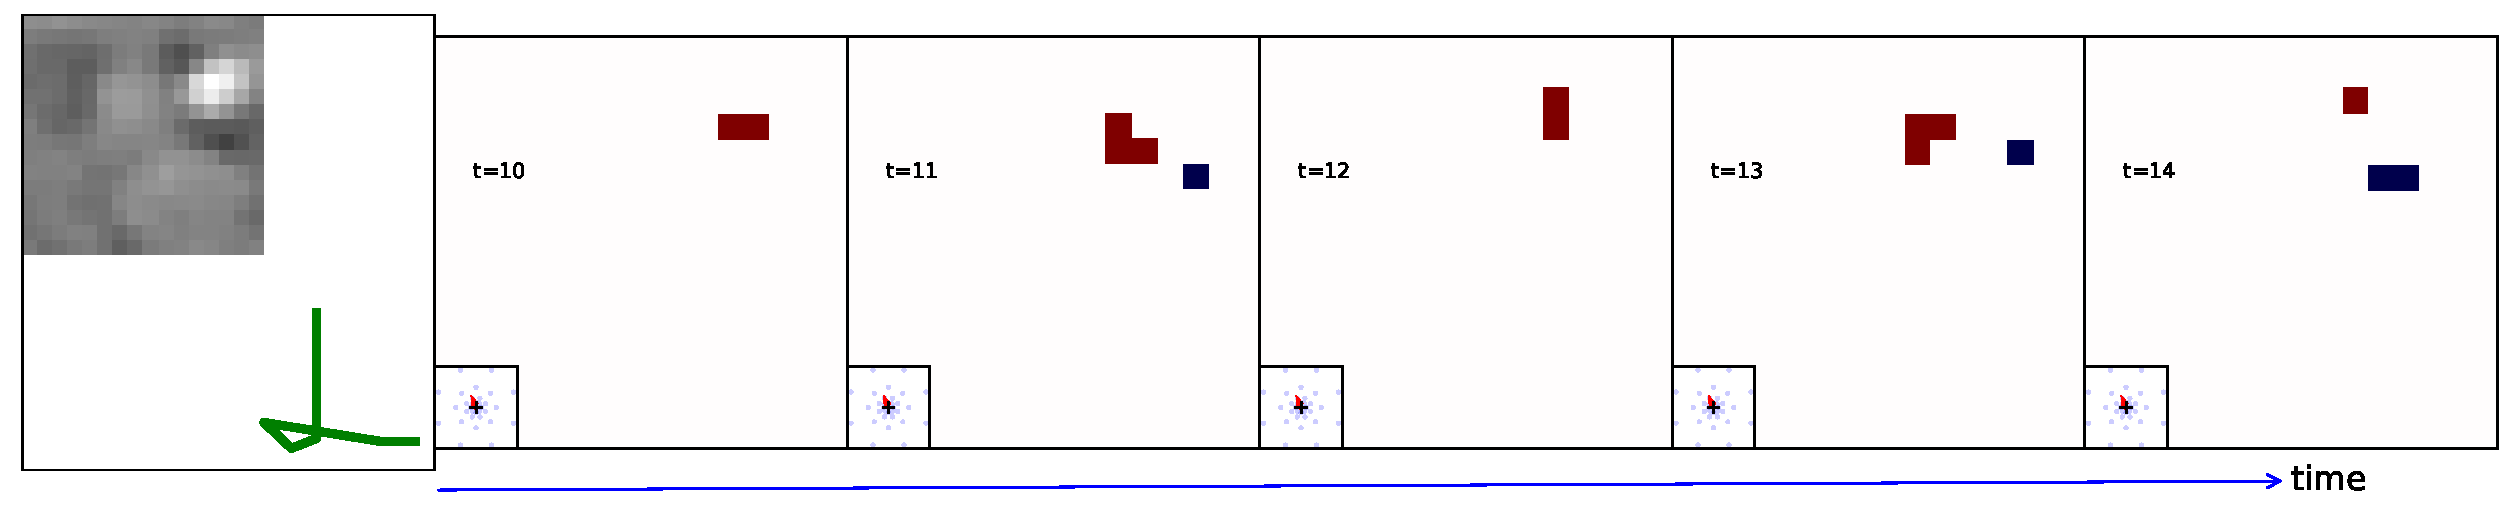
\includegraphics[width=0.95\linewidth]{figures/motion_task.pdf}
    \caption{
        {\bf - Motion Detection Task.} {\bf (Left)}~We use large natural images ($512\times512$) in which an aperture ($128\times128$) extracts a cropped image around the view axis. To mimic the effect of a saccadic eye movement, the view axis moves according to a stepwise random walk. We show an example path of the trajectory for $200$ time steps (green line). {\bf (Right)}~Snapshot of the synthetic event stream at different time steps. The dynamics of the sub-image as a function of time produces a naturalistic movie. This can be transformed into an event-based representation. Mimicking the retina, this representation encodes pixel-per-pixel proportional increases or decreases in luminance in the image, i.e. ON (red) and OFF (blue) events. In the lower left corner of the images, the translation vector is shown in red as one of the possible classes of motion. Note the change in the direction of motion between the second and third image.}
    \label{fig:motion_task}
\end{figure}
%%%-----------------------------------------------------------------
Once these eye trajectories are generated, we can apply them to a visual scene. % For this purpose, we selected a database of 10 natural grayscale images that are commonly used to study the statistics of natural images~\citep{olshausen_emergence_1996}. 
For this purpose, we selected a database of 600 natural images that were previously used to study the statistics of natural images~\citep{perrinet_edge_2015}. Note that these have been pre-processed to be in grayscale and to equalize (i.e., whiten) the energy in each frequency band. This process is known to occur in the retino-thalamic pathway~\citep{dan_efficient_1996}. These images are $256 \times 256$ in size, and we will extract sub-images of size $64 \times 64$ positioned around the center of gaze at each time step. We will discretize time in $1~\ms$ bins and produce movies of duration $N_T = 128~\ms$. To avoid boundary effects, we will randomly position the full trajectory in image space such that the subimage is translated using the position given by the trajectory at each time step without touching the borders. The translation is computed using a coordinate roll in the horizontal and vertical dimensions, followed by a sub-pixel translation defined in Fourier space~\citep{perrinet_sparse_2015}. Note that the magnitude of the displacement is relative to the time bin, and we have defined the velocity to correspond to a movement of one pixel per frame (i.e., per time bin).

To transform each movie into events, we compute a gradient image (initialized at zero) by adding the gradient of the pixels' intensity over two successive frames. If, on a specific pixel at that specific timestamp, the absolute value of this gradient exceeds a threshold, an event is generated. The event has either an OFF or ON polarity, respectively whether the gradient is negative or positive. This signed threshold value is then subtracted from the residual gradient image. When applied to the whole movie, the event stream is as a consequence similar to the output of a neuromorphic camera~\citep{rasetto_challenges_2022}, that is, a list of events defined by $x_\arank$ and $y_\arank$ (their position on the pixel grid), their polarity $\polev_\arank$ (ON or OFF) and time $\timev_\arank$  (\seeFig{motion_task}-(Right)). The goal here is to infer the correct motion solely by observing these events. 
% \note{ the task is full-field rigid translations, the model resolves it locally (analogy to the input from V1 to MT) }
%
%\subsection{Detecting event-based motifs using spiking neurons with heterogeneous delays}% model as a Logistic Regression with a temporal convolution}
%%%%-----------------------------------------------------------------
%%
%\begin{figure}%[t!]
%    \centering
%    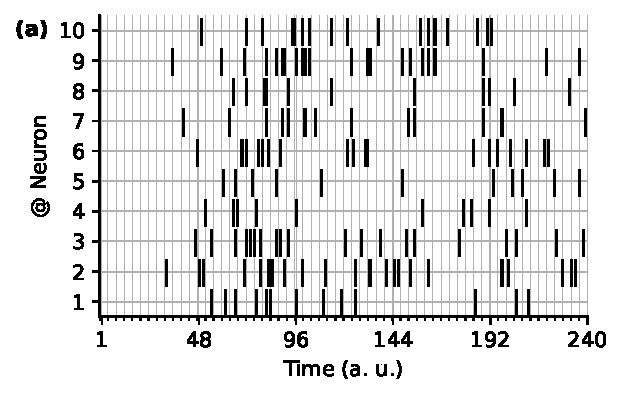
\includegraphics[width=0.490\linewidth]{figures/THC_1a_k.pdf}
%    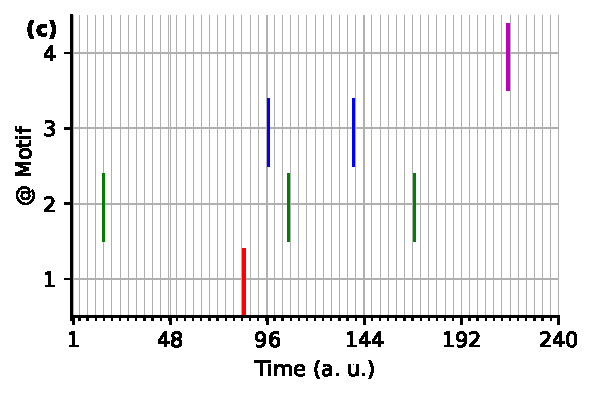
\includegraphics[width=0.490\linewidth]{figures/THC_1c.pdf}
%    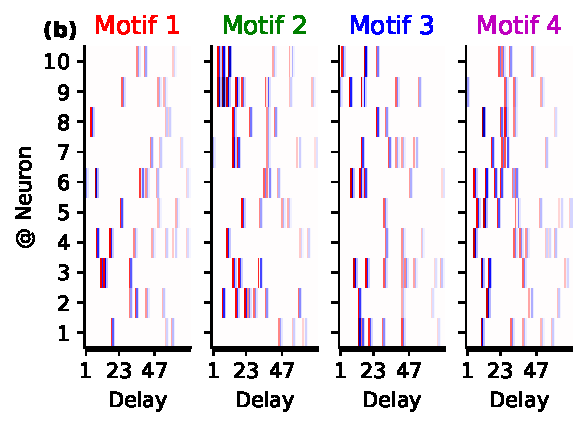
\includegraphics[width=0.490\linewidth]{figures/THC_1b.pdf}
%    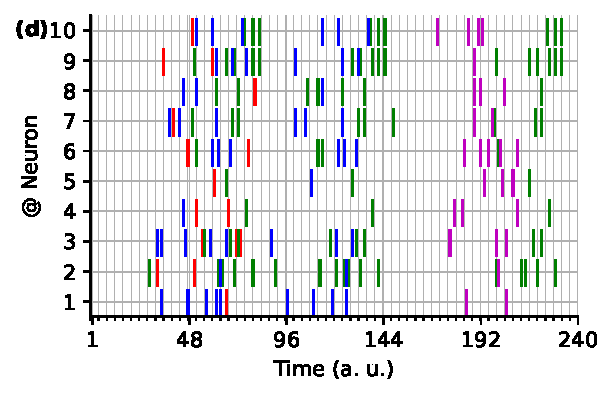
\includegraphics[width=0.490\linewidth]{figures/THC_1a.pdf}
%	    \caption{Detecting event-based motifs using spiking neurons with heterogeneous delays. 
%	    {\bf (a)}~Given a generic raster plot defined by a set of spikes occurring on specific neural addresses and at specific times, one may consider that this information consists of the repeated occurrence of precise spiking motifs. 
%	    {\bf (b)}~We show the motifs used in this example, each identified at the top by a different color. To each of the $10$ neural adresses and $71$ different possible delays is assigned an evidence of activation (red) or deactivation (blue). Note that each afferent may be connected with multiple weights at different delays.
%	    {\bf (c)}~The activation in time of the different motifs is then used to define a generative model for drawing a raster plot on the multi-unit address space: The propagation of the afferent information through these delays generates the raster plot seen in (a). 
%	    {\bf (d)}~The inversion of the generative model provides with a model which gives the predicted probability of occurrence of each motif at any time and which may be used to generate a spike as a Bernoulli trial. The detection model yields in this particular case with an exact identification of the occurrence of motifs. Knowing the results of this detection, one may for illustration purposes highlight them by different colors in the raster plots, showing that in this synthetic examples, all spikes can be annotated with each identified spiking motif. 
%	    }
%    \label{fig:model}
%\end{figure}
%% 
%\subsubsection{A generative model for raster plots}
%%
%In neurobiological recordings or in the sensory signal obtained from an event-based camera, any generic raster plot consists of a stream of \emph{spikes} or \emph{events} (see Figure~\ref{fig:model}-(a)). This can be formalized as a list of neural addresses and timestamps tuples $\event = \{(\presynaddr_\arank, \timev_\arank)\}_{\arank \in [1,\numevent]}$ where $\numevent \in \mathbb{N} $ is the total number of events in the data stream and the rank $\arank$ is the index of each event in the list of events. Events are typically ordered by their time of occurrence. Each event has a time of occurrence $\timev_\arank$  and an associated address $\presynaddr_\arank$ (which is typically in the form $(x_\arank, y_\arank, \polev_\arank)$ for event-based cameras). This defines an address space $\presynaddrspace$ which consists of the set of possible addresses. In a neurobiological recording, this can be the identified set of neurons. For event-based cameras, it is denoted by $[1, \Nx]\times[1, \Ny] \times [1, \Npol] \subset \mathbb{N}^3$ where $(\Nx, \Ny)$ is the size of the sensor in pixels and $\Npol$ is the number of polarities ($\Npol=2$ for the ON and OFF polarities coded in event-based cameras). 
%
%% This raster plot is generated by spiking neurons which are defined on the one hand by the equations governing the evolution of its membrane potential dynamics on its soma and on the other hand by the characterization of the synaptic contacts on its dendritic tree, or on the sensory processes (such as the pixel on the sensor of a camera, or the photoreceptors in the retina). A classical characterization consists in detailing the synaptic weights of each synaptic contact on the dendritic tree, the so-called weight matrix. A more detailed description of these synaptic contacts reveals the added importance of heterogeneous delays, i.e., the precise timing from one afferent neuron's firing to its arrival in the soma, and how this changes the network's dynamics~\citep{izhikevich_polychronization_2006}. In that description, we can parameterize each neuron by the set of tuples defining both the weight and the delay of each synaptic contact. As a consequence, a set of input presynaptic spikes $\event$ will be processed by the dendrites defined by this synaptic set and notably by the respective delays, which will multiplex in time all events. 
%
%Let's formalize a layer of spiking neurons with heterogeneous delays (HD-SNN). Each neuron $\postsynaddr \in \postsynaddrspace$  connects to presynaptic afferent from $\presynaddrspace$. In biology, a single cortical neuron has generally several thousands of synapses. Each synapse may be defined by its synaptic weight and its delay, that is, the time it takes for one spike to travel from the presynaptic neuron's soma to that of the postsynaptic neuron. A postsynaptic neuron $\postsynaddr \in \postsynaddrspace$ is then described by the synaptic weights connecting it to a presynaptic afferent from $\presynaddrspace$ but also by the set of possible delays. Note that a neuron may contact an afferent neuron with multiple different delays. Scanning all neurons $\postsynaddr$, we thus define the full set of $\Nsyn$ synapses, 
%as  $\synapse = \{(\presynaddr_\ranksyn, \postsynaddr_\ranksyn, \synapticweight_\ranksyn, \synapticdelay_\ranksyn)\}_{\ranksyn \in [1,\Nsyn]}$, where each synapse is associated to a presynaptic address $\presynaddr_\ranksyn$, a postsynaptic address $\postsynaddr_\ranksyn$,  a weight $\synapticweight^\ranksyn$, and a delay $\synapticdelay_\ranksyn$. This defines the full connectivity of the HD-SNN model. Of interest is to define the receptive field of a postsynaptic neuron $\synapse^\postsynaddr =  \{(\presynaddr_\ranksyn, \postsynaddr_\ranksyn, \synapticweight_\ranksyn, \synapticdelay_\ranksyn) \| \postsynaddr_\ranksyn=\postsynaddr\}_{\ranksyn \in [1,\Nsyn]} $, or the emitting field of a presynaptic neuron $\synapse_\presynaddr =  \{(\presynaddr_\ranksyn, \postsynaddr_\ranksyn, \synapticweight_\ranksyn, \synapticdelay_\ranksyn) \| \presynaddr_\ranksyn=\presynaddr\}_{\ranksyn \in [1,\Nsyn]}$. As a consequence, an event stream which evokes neurons in the presynaptic address space is multiplexed by the synapses into a new event stream which is defined by the union of the sets generated by each emitting field from the presynaptic space: 
%$ \cup_{\arank \in [1,\numevent]} \{ \{(\postsynaddr_\ranksyn, \synapticweight_\ranksyn, \timev_\arank + \synapticdelay_\ranksyn) \}_{ \ranksyn \in \synapse_{\presynaddr_\arank}} \}$. This new stream of events is by nature ordered in time as events reach the soma of post-synaptic neurons. In particular, when post-synaptic neurons are activated on their soma by this spatio-temporal motif, the discharge probability will increase, notably when these spikes converge on the soma in a synchronous manner. 
%% \note{ TODO: show why this formula implements a polychrony detector }
%
%% \note{ éclaircir }
%
%Taking the argument the other way around, one may from a generative model for generic raster plots. Indeed, any spike in the presynaptic address space is generated by sensory neurons (for instance photoreceptors in the retina, sensors in a CMOS chip) or by afferent spiking neurons. In the latter case, these are connected to the spiking cell by a set of weights and delays, whose structure is stable relatively to the coding timescale. When these connections are high and sparsely distributed, this firing will cause a specific temporal motif. Another example is given for the barn owl auditory system: As it hears the sound of a mouse, this sound will generate a specific spiking response in both ears, and specifically, the precise timing between the signal generated by the left relative to the right ear can be for instance used to determine the position of the prey~\citep{goodman_spike-timing-based_2010}. Overall, these examples show that raster plots may be considered as a mixture of the effects of different elementary causes, and that each event triggers a specific spatio-temporal spiking motif. 
%%
%\subsubsection{Detecting spiking motifs}
%%: Detection model
%
%From the perspective of simulating such event-based computations on standard CPU- or GPU-based computers, it is useful to transform this event-based representation into a dense representation. Indeed, we may transform any event-based input as the boolean matrix $A \in \{0, 1 \}^{N\times T}$, where $N$ is the number of neurons in $\presynaddrspace$ and $T$ is the number of time bins. In this simplified model, we will consider that heterogeneous delays are limited in range such that the synaptic set can be represented by the dense matrix $\kernel^\postsynaddr$ giving for each neuron $\postsynaddr$ the weights as a function of presynaptic address and delay: $\forall {\ranksyn \in [1,\Nsyn^\postsynaddr]}, \kernel^\postsynaddr(\presynaddr_\ranksyn^\postsynaddr, \synapticdelay_\ranksyn^\postsynaddr) = \synapticweight_\ranksyn^\postsynaddr$. 
%The probability of firing of a neuron $a$ at a given time $t$ can be understood as a Bernoulli trial whose (only) parameter is a bias $p(t, a) \in [0, 1]$. Assuming that the presence of spiking motifs conditions the probability on all efferents, the logit (inverse of the sigmoid) of this probability bias can be written as the sum of the logit of each of these factors, whose values are defined by the corresponding weights. Spiking motifs may be activated independently and at random times, such that  we write this activity as $B(b, t)=1$ if $b$ is activated at $t$ and else $B(b, t)=0$. We can thus write the probability bias as the accumulated evidence given these factors as 
%\begin{equation*}
%p(t, a) = \sigma\big(W_0 + \sum_{b, t} B(b, t) \cdot W_b(a, t-d) \big)  
%\end{equation*}
%where $\sigma$ is the sigmoid function. We will further assume that the weights are balanced (their mean is zero) and that $W_0$ is a bias such that $p_0=\sigma(W_0)$ is the average background firing rate. Conveniently, one can write this summation as a one-dimensional temporal convolution operator such that we may simply write
%\begin{equation*}
%p = \sigma(W_0 + B \ast W )
%\end{equation*}
%where  $p\in [ 0, 1]^{N\times T}$ and $B\in \{0, 1\}^{M\times T}$ is the raster plot corresponding to the temporal activation of the PGs. Finally, we obtain the raster plot $A\in \{0, 1\}^{N\times T}$ by drawing spikes using independent Bernoulli trials $A \sim \mathcal{B}(p)$. Note that, depending on the shape of the kernels, the generative model can model a discretized Poisson process, generate rhythmic activity or more generally propagating waves. This formulation thus defines a simple generative model for raster plots as a combination of independent PGs. 
%
%Using this dense representation, the counting defined above becomes:
%\begin{equation*}
%\mathcal{C}^\postsynaddr(a,t)
%= \sum_{\presynaddr, \synapticdelay_\ranksyn^\postsynaddr} \kernel^\postsynaddr(\presynaddr_\ranksyn^\postsynaddr, \synapticdelay_\ranksyn^\postsynaddr) \cdot A(\presynaddr, \timev-\synapticdelay_\ranksyn^\postsynaddr)
%\end{equation*}
%%
%This shows that $\mathcal{C}^\postsynaddr$ is a temporal convolution of the dense representation of the event stream with the dense kernels formed by the set of synapses:  $\mathcal{C}^\postsynaddr = \kernel^\postsynaddr \ast A$.
%This well-known computation defines a time-invariant, differentiable measure which is very efficiently implemented for GPUs and which we will use for learning the classification of different motifs in the event stream.
%%
%
%\note{formalize the following:}
%More generally, every cause may be considered as occurring independently and one might write the generative model for the generation of the presynaptic events as:
%
%
%Using this formalization, one might now deduce an optimal algorithm for the detection of such temporal motifs.
%
%
%By discretization of time (with here an arbitrary unitary time unit), we can also define the dendrite as a matrix giving the weight corresponding to the different delays $d \in [0, D]$ (where $D$ is the maximum delay) on different pre-synaptic addresses $a \in [1, N]$ defining the list of the $N$ dendrites. We will denote as $W(a, d)$ these weights.
%
%
%Following the observations of~\citet{izhikevich_polychronization_2006}, let us assume that such precise discharge motif defines a polychronous group (PG). Assuming that we know there exists $M$ such groups, we will define as $b \in [1, M]$ the address of a PG and as $W_b$ the corresponding weight matrices. This allows then to derive a generative model for raster plots (see Figure~\ref{fig:model}-(b)).

% 
%This generative model defined above allows to determine this inference model for guessing sources $B$ when observing a raster plot $A$. This assumes that we know the spiking motifs as defined by the $W_b$ matrices. The underlying metric is the binary cross-entropy, as used in the logistic regression model. In particular, if we consider kernels with similar decreasing exponential time profile, we can prove that this is similar to the method of~\citet{berens_fast_2012}. In our specific case, the difference is that the regression is performed in both dendritic and delay space by extending the summation using a temporal convolution operator. Using this forward model, it is possible to estimate the logit (inverse of a sigmoid) $\hat{B}(b, t)$ for the presence of a PG of address $b$ and at time $t$ by using the transpose convolution operator. Equivalently, this consists in using the emitting field $\synapse_\presynaddr$ of presynaptic neurons in place of the receptive field $\synapse^\postsynaddr$ of postsynaptic neurons. It thus comes that when observing $A$, then one may infer $\hat{B} = A \ast W^T$ and select the most activated items. This assumption hold as long as the kernels are uncorrelated, a condition which is met here numerically by chosing a relatively sparse set of synapses (approximately $1\%$ of active synapses).


%\subsubsection{Implementation using spiking neurons with heterogeneous delays}
%
% The activation function of our spiking neural is a softmax function implementing a form of  Multinomial Logistic Regression (MLR)~\citep{grimaldi_robust_2022}, in analogy to a spiking Winner-Take-All network~\citep{nessler_bayesian_2013}. 
%It transforms this list of weights into a probability with the following formula:
%$
%Pr(k=\postsynaddr \; \vert \; \timev) =
%\frac 1 Z
%{\exp  (\mathcal{C}^\postsynaddr(\timev) +\bias^\postsynaddr) }
%$ 
%where $\mathcal{C}^\postsynaddr(\timev) = \sum
%\activeweights^\postsynaddr(t)
%$ is the sum of the synaptic weights and $\bias^\postsynaddr$ is the bias linked to neuron $\postsynaddr$. 
%In particular, we expect that some specific motifs may become tightly synchronized as they reach the basal dendritic tree, leading to a high postsynaptic activity which makes it progressively more likely to generate an output spike.
%%
%
% \note{say that it is effortless in biology but difficult on conventional computers}
% In our MLR model with $\Nclass=\Nspeed$ classes, a probability value is predicted for each event at address $\presynaddr_\arank$ and at time $\timev_\arank$ as a softmax function of the linear combination of the list of events on the basal dendrite of a neuron $\postsynaddr$ in association to a specific class. The linear combination can be defined by a set of synapses $\synapse^\postsynaddr$ as described in the heterogeneous delays model. 
%
%\subsubsection{Performance on synthetic data}
%%
%\begin{figure}%[t!]
%    \centering
%    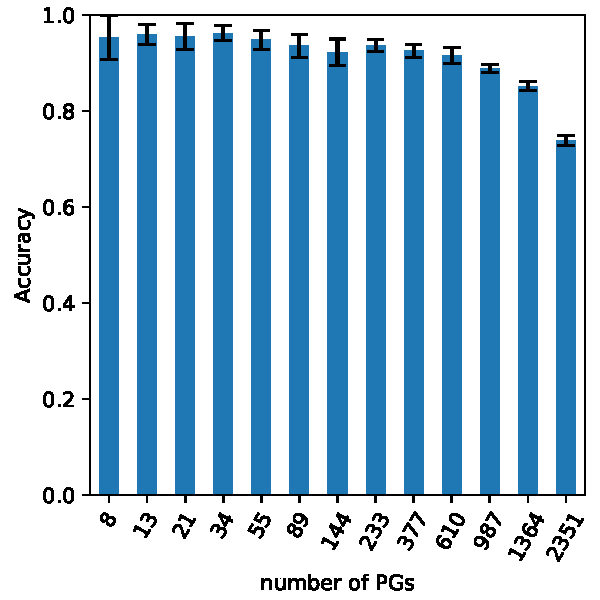
\includegraphics[width=0.490\linewidth]{figures/THC_N_PGs.pdf}
%    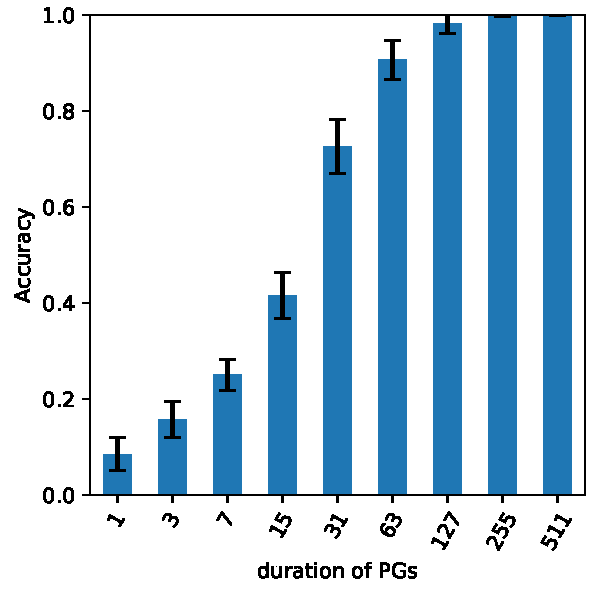
\includegraphics[width=0.490\linewidth]{figures/THC_N_PG_time.pdf}
%	    \caption{Detecting event-based motifs using spiking neurons with heterogeneous delays. 
%	    {\bf (a)}~Accuracy of detection as a function of the number of kernels.
%	    {\bf (b)}~Accuracy of detection as a function of the temporal depth $D$ of kernels among $M=144$ kernels.
%	    }
%    \label{fig:model_results}
%\end{figure}
%
%To quantify the efficiency of this operation, we generated $M=144$ synthetic spiking motifs as random independent kernels over $128$ presynaptic inputs and $D=71$ possible delays. We drew random independent instances of $B$ with a length of $T=1000$ time steps and with on average $1.0$ occurrences in each draw. This allowed us to generate raster plots which we use to infer $\hat{B}$. We compute the accuracy as the rate of true positive detections (both for inferring the address and its exact timing) and observe on average $\approx 98\%$ correct detections. We further extended this result by showing how the accuracy would evolve as a function of the number of simultaneous PGs, while keeping the same frequency of occurrence. We show in Figure~\ref{fig:model_results}~(a) that the accuracy of finding the right PG is still above $80\%$ accuracy with more than $1364$ overlapping PGs. Moreover, we show in Figure~\ref{fig:model_results}~(b) that (with $M=144$ PGs fixed) the accuracy increases notably as the temporal depth $D$ of the PG kernel increased, demonstrating quantitatively the computational advantage of using heterogeneous delays. These results were obtained while assuming that we know $W$. However, this is in general not the case, for instance when observing the raster plot of a population of neurons. In the following, we will define a generic visual task and determine a learning algorithm to solve that challenging task. %Inspired by the k-means algorithm, it is possible to devise a self-supervised learning algorithm. Our preliminary results show that it is possible to retrieve PGs embedded in the data, yet that further analysis is necessary to improve the convergence of the algorithm. In particular, it seems promising to use a sparseness constraint in the inference mechanism such as to remove spurious correlations in the inference.
%
% \subsection{Description of the model}
%%%-----------------------------------------------------------------
\subsection{The Heterogeneous Delays SNN (HD-SNN) model}
%----------------------------%
%
\begin{figure}%[t!]
    \centering
    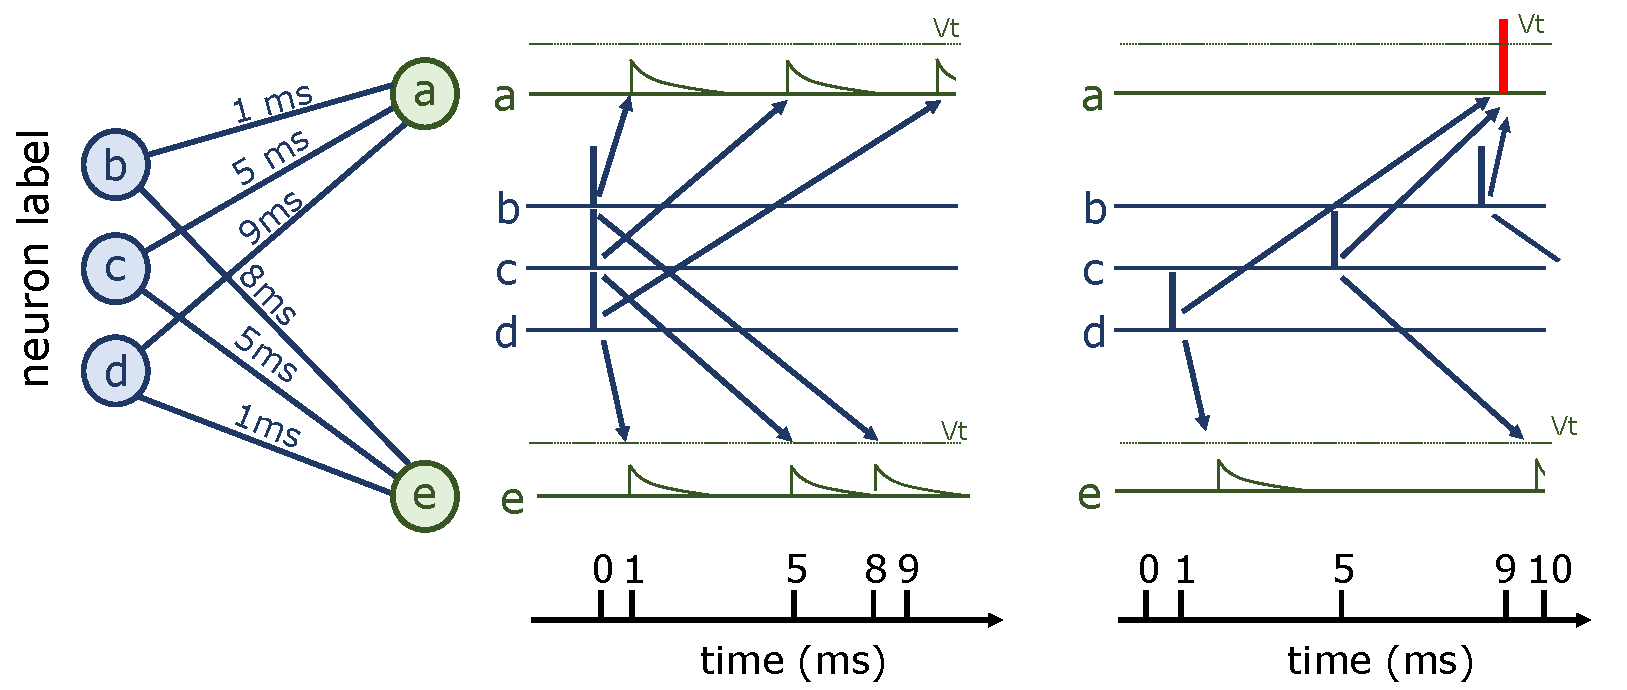
\includegraphics[width=0.980\linewidth]{figures/izhikevich.pdf}%png}% https://www.overleaf.com/5625872443qpcwrkssgbsf
      \caption{\textbf{Core mechanism of the HD-SNN model.} \textit{(Left)}~In this example inspired by the polychronization model~\citep{izhikevich_polychronization_2006}, three presynaptic neurons denoted \textit{b}, \textit{c} and, \textit{d} are fully connected to two post-synaptic neurons \textit{a} and \textit{e}, with different delays of respectively $1$, $5$, and $9~\ms$ for \textit{a} and  $8$, $5$, and $1~\ms$ for \textit{e}. \textit{(Middle)}~If three synchronous pulses are emitted from presynaptic neurons, this will generate post-synaptic potentials that will reach \textit{a} and \textit{e} asynchronously because of the heterogeneous delays, and they may not be sufficient to reach the membrane threshold in either of the post-synaptic neurons, therefore no spike will be emitted as this is not sufficient to reach the membrane threshold of the post synaptic neuron, so no output spike is emitted.
      %at these different delays, and these may not be sufficient to generate a spike in either neuron.
      \textit{(Right)}~If the pulses are emitted from presynaptic neurons such that, taking into account the delays, they reach the post-synaptic neuron \textit{a} at the same time (here, at $t=10~\ms$),  the post-synaptic potentials evoked by the three pre-synaptic neurons sum up, causing the voltage threshold to be crossed and thus to the emission of an output spike (red color), while none is emitted from post-synaptic neuron \textit{e}. Figure reproduced from~\cite{grimaldi_precise_2023} under a CC-BY licence.
       }
    \label{fig:izhikevich}
  \end{figure}
  % 
  %----------------------------%

In neurobiological recordings or in the sensory signal obtained from an event-based camera, any generic raster plot consists of a stream of \emph{spikes} or \emph{events}. This can be formalized as a list of neural addresses and timestamps tuples $\event = \{(\presynaddr_\arank, \timev_\arank)\}_{\arank \in [1,\numevent]}$ where $\numevent \in \mathbb{N} $ is the total number of events in the data stream and the rank $\arank$ is the index of each event in the list of events. Events are typically ordered by their time of occurrence. Each event has a time of occurrence $\timev_\arank$ and an associated address $\presynaddr_\arank$. This defines an address space $\presynaddrspace$ which consists of the set of possible addresses. In a neurobiological recording, this can be the identified set of neurons. For event-based cameras, this can be defined as $[1, \Npol] \times [1, \Nx]\times[1, \Ny] \subset \mathbb{N}^3$ where $\Npol$ is the number of polarities ($\Npol=2$ for the ON and OFF polarities coded in event-based cameras) and $(\Nx, \Ny)$ is the size of the sensor in pixels. As such, an address $\presynaddr_\arank$ is typically in the form $(\polev_\arank, x_\arank, y_\arank)$ for event-based cameras.

Let's formalize the heterogeneous delays spiking neural network (HD-SNN). Each neuron $\postsynaddr \in \postsynaddrspace$ connects to presynaptic afferents from $\presynaddrspace$. In biology, a single cortical neuron has generally several thousands of synapses. Each synapse may be defined by its synaptic weight and its delay, that is, the time it takes for one spike to travel from the presynaptic neuron's soma to that of the postsynaptic neuron. A postsynaptic neuron $\postsynaddr \in \postsynaddrspace$ is then described by the synaptic weights connecting it to a presynaptic afferent from $\presynaddrspace$ but also by the set of possible delays. Note that a neuron may contact an afferent neuron with multiple different delays. Scanning all neurons $\postsynaddr$, we thus define the full set of $\Nsyn$ synapses, 
as  $\synapse = \{(\presynaddr_\ranksyn, \postsynaddr_\ranksyn, \synapticweight_\ranksyn, \synapticdelay_\ranksyn)\}_{\ranksyn \in [1,\Nsyn]}$, where each synapse is associated to a presynaptic address $\presynaddr_\ranksyn$, a postsynaptic address $\postsynaddr_\ranksyn$, a weight $\synapticweight_\ranksyn$, and a delay $\synapticdelay_\ranksyn$. This defines the full connectivity of the HD-SNN model. 

Of interest is to define the receptive field of a postsynaptic neuron $\synapse^\postsynaddr =  \{(\presynaddr_\ranksyn, \postsynaddr_\ranksyn, \synapticweight_\ranksyn, \synapticdelay_\ranksyn) \| \postsynaddr_\ranksyn=\postsynaddr\}_{\ranksyn \in [1,\Nsyn]}  \subset \synapse$, or the emitting field of a presynaptic neuron $\synapse_\presynaddr =  \{(\presynaddr_\ranksyn, \postsynaddr_\ranksyn, \synapticweight_\ranksyn, \synapticdelay_\ranksyn) \| \presynaddr_\ranksyn=\presynaddr\}_{\ranksyn \in [1,\Nsyn]} \subset \synapse$. As a consequence, a postsynaptic neuron $\postsynaddr$ receives an event stream which is multiplexed by the synapses of its receptive field. It results in a weighted event stream for each  postsynaptic neuron $\postsynaddr$: 
\begin{equation}\label{eq:stream_b}
\event_\postsynaddr = \{(\presynaddr_\arank, \timev_\arank+\synapticdelay_\ranksyn) \| \presynaddr_\arank = \presynaddr_\ranksyn \}_{\arank \in [1,\numevent], \ranksyn \in \synapse^\postsynaddr}
\end{equation}
Unlike the binary stream of events from the signal as input, the postsynaptic neurons receive a weighted stream of event such that for each event $\arank$ its value is $\synapticweight_\arank = \synapticweight_\ranksyn$ when $\presynaddr_\arank = \presynaddr_\ranksyn$. This new stream of events is ordered in time in biology as events reach the soma of post-synaptic neurons but should be reordered in simulations. Crucially, when post-synaptic neurons are activated on their soma by a specific spatio-temporal motif which is imprinted in the set of synapses, the discharge probability will increase, notably when these spikes converge on the soma in a synchronous manner (see Figure~\ref{fig:izhikevich}). This model is defined in this subsection in all generality and the activation function of the neurons of the HD-SNN can be selected among the whole range of spiking neuron response functions. In the next subsection we describe an implementation of our model adapted for the motion detection task. 
%
% \note{I can make a small figure with event streams of different colors for the input one, the multiplexed one etc and the response in the bottom}
%
\subsection{Application of HD-SNN to the motion detection task}
%
From the perspective of simulating such event-based computations on standard CPU- or GPU-based computers and then using parallel computing, it is useful to transform this event-based representation into a dense representation. Indeed, by discretization of time, we may transform any event-based input as a boolean matrix $A \in \{0, 1 \}^{\Npol \times \Ntime \times \Nx \times \Ny}$, defined for all polarities $p$, times $t$ and space coordinates $x$ and $y$. The values are by definition equal to zero except at the occurences of events: $\forall \numevent \in \mathbb{N}$, $A()=1$

$\event = \{(\presynaddr_\arank, \timev_\arank)\}_{\arank \in [1,\numevent]}$ where $\numevent \in \mathbb{N} $ is the total number of events in the data stream and the rank $\arank$ is the index of each event in the list of events. Events are typically ordered by their time of occurrence. Each event has a time of occurrence $\timev_\arank$ and an associated address $\presynaddr_\arank$ (which is typically in the form $(x_\arank, y_\arank, \polev_\arank)$ for event-based cameras). 


To benefit from invariance to location observed in CNN and to simplify the implementation of the model, one assumes that kernels should be similar across different positions and define a convolution operator. % The characteristics of the kernels are shared among one class of neurons such that $\forall i,j \in [1, N_\class]^2, \; \kernel^i_\class = \kernel^j_\class$. 
% Here, we will consider that heterogeneous delays are limited in range
In particular, the whole synaptic set can be represented as a one kernel for each class $\class$ of the supervision task as the dense matrix $\kernel_\class$ of size $(\Npol, \Ktime, \Kx, \Ky)$, where  $\Ktime$ is the number of delays and $\Kx$ and $\Ky$ are the number of pixels in both spatial dimensions. To keep an analogy with the HD-SNN model, for each neuron $\postsynaddr$ of position $(x, y)$ and class $\class$, $\kernel_\class$ gives the weights as a function of presynaptic address and delay: $\forall {\ranksyn \in \synapse^\postsynaddr}, \kernel_\class(\presynaddr_\ranksyn, \synapticdelay_\ranksyn) = \synapticweight_\ranksyn$. Therefore, if we make the approximation that one neuron integrates only on the temporal window given by its variety of synaptic delays, the integration of the spike train as input can be formalized by a 3D convolution operation. The longest synaptic delay defines the depth of the kernel $\kernel^\postsynaddr$ and all possible delays associated to the different presynaptic addresses are represented. Using this dense representation, the processing of $A$ by the model can be written as:
\begin{equation}\label{eq:kernel_b}
\forall x, y, \timev, \; \;
\mathcal{C}_\class(x, y, \timev)
= \sum_{p, \delta_x, \delta_y, \synapticdelay} \kernel_\class(p, \delta_x, \delta_y, \synapticdelay) \cdot A(p, x - \delta_x, y - \delta_y, \timev-\synapticdelay)
\end{equation}
% The computational brick used in equation~\eqref{eq:kernel_b} can be extended to every position, in space and time, of the boolean matrix $A$:
% \begin{equation}\label{eq:conv}
% \forall \presynaddr \in \presynaddrspace, \forall \timev \in T, \; \;
% \mathcal{C}_\class(\presynaddr,\timev)
% = \sum_{\ranksyn  \in [1, N_{\synapse^\postsynaddr}]} \kernel_\class(\presynaddr_\ranksyn, \synapticdelay_\ranksyn) \cdot A(\presynaddr, \timev-\synapticdelay_\ranksyn)
% \end{equation}
This shows that $\mathcal{C}_\class$ is a spatiotemporal convolution of the dense representation of the event stream with the dense kernels formed by the set of synapses:  $\mathcal{C}_\class = \kernel_\class \ast A$ (see Figure~\ref{fig:model} for an illustration). Note that to remain within the framework of a causal calculation, the kernels are shifted in time such that only past information gives an answer at the present time.
This well-known computation defines a differentiable measure which is very efficiently implemented for GPUs and which we will use for learning the classification of different motifs in the event stream.

The same type of spatiotemporal filtering is used as a preprocessing stage of a pattern recognition algorithm~\cite{ghosh_spatiotemporal_2019}. And in \cite{sekikawa_constant_2018}, an efficient 3D convolutional algorithm succeeds a motion estimation task. By assuming a locally constant velocity, the 3D kernel can be decomposed into a 2D kernel representing the shapes and a 3D kernel representing the velocity. Here, we keep the analogy with spiking neurons, and we try to use as few heuristics as possible to observe the emergence of spiking motifs in the spatiotemporal kernels. If so, this precise spatiotemporal patterns prove to be of interest for neural computations and one can assume that biological neurons make use of this information as well. 
% \note{plus de biblio sur la motion detection/segmentation ou optique flow avec les events? (reviewer 2)}
The 3D convolution represents the linear integration of the spike train as input. The activation function of our model is a softmax function implementing a form of Multinomial Logistic Regression (MLR)~\citep{grimaldi_robust_2022}, in analogy to a spiking Winner-Take-All network~\citep{nessler_bayesian_2013}. In our MLR model, a probability value, for each class (i.e. each motion direction), is predicted for each event at position $x, y$ and at time $\timev$ as a softmax function of the linear combination of the list of events. % on the basal dendrite of a neuron $\postsynaddr$ in association to a specific class. The linear combination can be defined by a set of synapses $\synapse^\postsynaddr$ as described in the HD-SNN model. 
Using the kernels, it transforms the input raster plot into a probability with the following formula:
\begin{equation}\label{eq:mlr}
    \forall x, y, \timev, \forall \class \in [1, N_\class], \; \;
Pr(k=\class \; \vert \;  x, y, \timev) =
\frac {\exp  (\mathcal{C}_\class(x, y, \timev) +\bias_\class) }{Z(x, y, \timev)}
\end{equation} 
where $Z(x, y, \timev)=\sum_{\class \in [1, N_\class]} \exp  (\mathcal{C}_\class(x, y, \timev) +\bias_\class)$ is the partition function and  $\bias_\class$ is the bias linked to class $\class$. 
In particular, we expect that some specific motifs may become tightly synchronized as they reach the basal dendritic tree, leading to a high postsynaptic activity which makes it progressively more likely to generate an output spike. The spiking output of the model corresponds to an event with the highest probability class. 

Once explained the general framework used to solve the ecological task described in section~\ref{sec:task}, we can add some heuristics based on neuroscientific observations to constrain our model and its strategies to solve the task. Note that the general framework is the same as the one presented in~\cite{grimaldi_learning_2022} and that, appart from the task to solve and a deeper analysis of the results, these priors, inspired by neuroscience, are the main methodological differences with this previous study. We set \note{arbitrarily} the size of the kernels to $(9, 17, 17)$ and define as many classes as the number of motion direction: $N_\class = 8$. Because receptive fields of biological neurons are mainly circular and can be more or less elongated, we apply a circular mask on the spatial dimensions of the kernels. And because the synaptic delay is linked, by physical principles, to the distance between the presynaptic neuron and the postsynaptic one, we apply a linear mask on the temporal axis such that the connectivity depends on the delay: the lower the delay the lower the circular mask radius (see Figure~\ref{fig:kernels} for an illustration). The second heuristics is based on the observation that biological neurons have a sparse spiking activity. From this observation, we set an output firing rate for the layer of spiking neurons in order to make a sparse selection of the events at which the model makes a decision. It results in the selection of the coefficients with the maximum likelihood value. Therefore, we will only select a given proportion of the most active cells, which we set here to $.01\%$ of all output voxels. This threshold was found using cross-validation and future work should automate how this may be determined for various datasets. Given a stimulus input, the model thus yields a spike output in the postsynaptic address space.

% \note{describe the heuristics inspired by neuroscience}

% \note{describe the parameters of the model}

\begin{figure}%[h!]%[ht!]
    \centering
    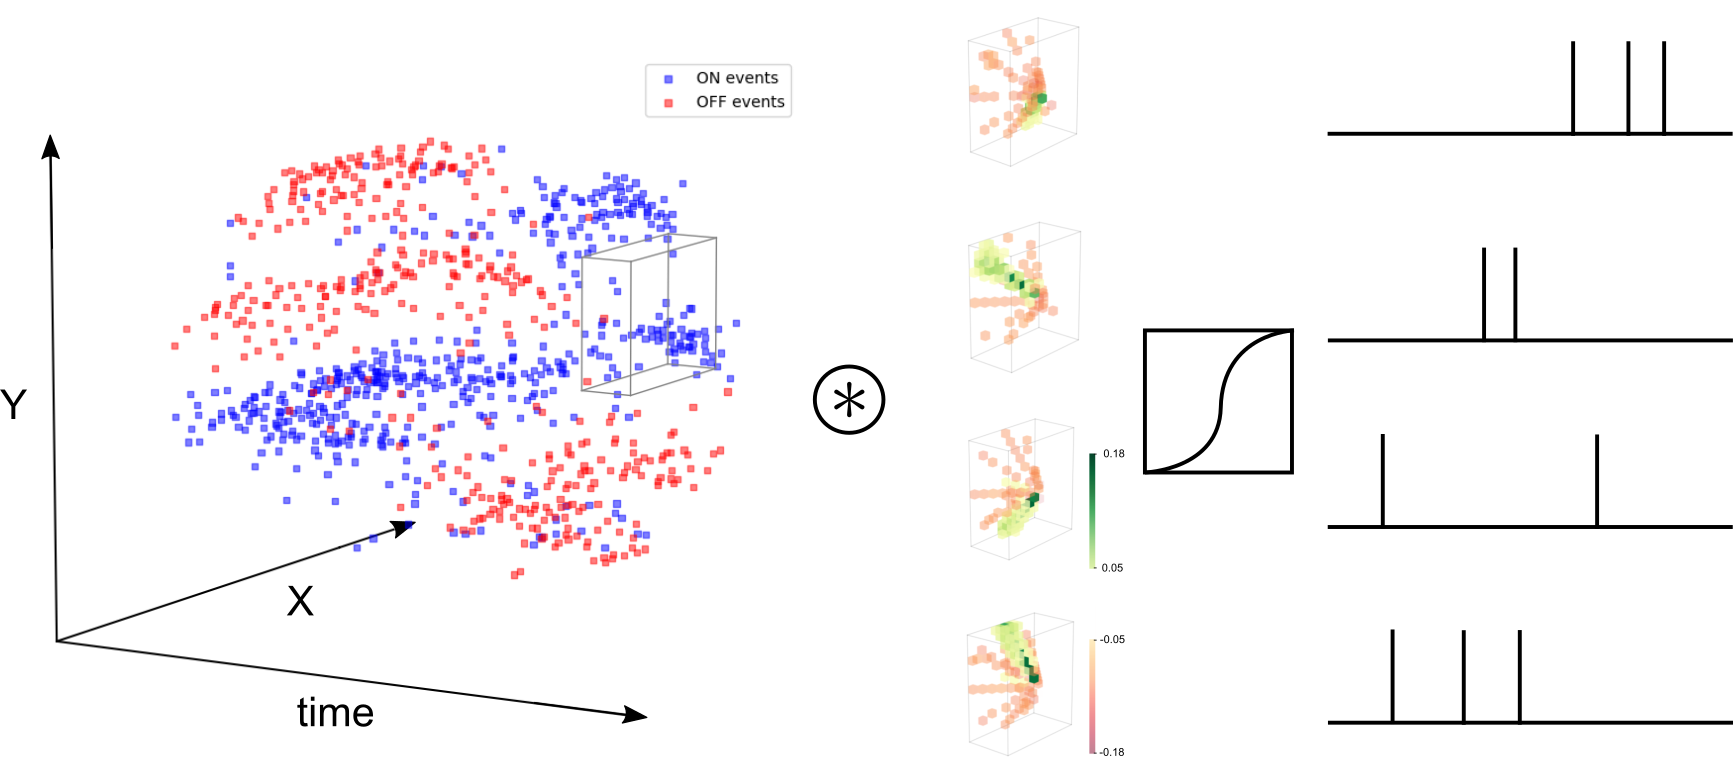
\includegraphics[width=\linewidth]{figures/HD-SNN.png}
    \caption{
    \textbf{- HD-SNN illustration. From left to right:} A 3D representation of the event stream as output of the DVS. A 3D convolution is applied, on the dense representation of the input, along the $X$ and $Y$ spatial axes (defining the DVS pixel grid) and the temporal axis. There are as many kernels as the possible number of motion classes in the recording. For clarity, only $4$ kernels are illustrated and some weights are not represented in the voxel grid. For each voxel on the dense representation of the event stream as input, the output of the 3D convolution is processed by the non-linearity of the MLR model (i.e. softmax function). The output of the MLR gives a probability for each class, associated to a specific kernel, to emit an output event, or spike. With an appropriate spiking mechanism, here a winner-takes-all, we obtain, as output of the HD-SNN model, a new spike train with the different spikes associated to a specific motion class. }
    \label{fig:model}
\end{figure}

\subsection{Supervised learning of the motion detection task}
%
Since the model is fully differentiable, we can now implement a semi-supervised learning rule. The loss function of the MLR model is the binary cross-entropy on the output of the classification layer. Supervision was implemented using the input binary events as defined above and the motion direction labels as the desired output. The labels were defined at each time point as a one-hot encoding of the current motion in the channel corresponding to the current motion for all positions. As in this semi-supervised context, the label is known, but the timing is not, we used a selection of the temporal support in an unsupervised manner. It is important to note that we weighted the cost function by considering only active cells, such that the error is only back propagated to the spatial locations of these most active cells. This is reminiscent of previous methods solving this problem using a Winner-Takes-All mechanism~\citep{masquelier_unsupervised_2007}. Simulations are performed with the PyTorch library using gradient descent with Adam (for $2^{12}$ movies and a learning rate of $10^{-5}$). We demonstrated in a previous work that this type of learning algorithm can be assimilated to a Hebbian learning mechanism~\cite{grimaldi_robust_2022}.  
%
Finally, the output of the MLR model is an event-based representation predicting at each position and at each time the probability of each motion. Such an output gives a form of optical flow that can be exploited for non-rigid motions, but we have defined here, for simplicity, an evaluation method that applies to our task with a full field motion. We have shown above that when different independent observations (here, the estimated motion at different spatial locations) are recognized as having a common cause (here, the rigid motion of the image), then an optimal estimate of the logit of this probability is the sum of the logits of the independent probabilities. By taking the logit of the probability of the output given by the model, we can therefore calculate the probability of the output. This allows one to calculate the accuracy (as the percentage of times the motion is accurately predicted) or the squared error of the velocity estimate given by the average estimate. 
These calculations are performed on a different input dataset than the one used in the training or validation steps. The complete code to reproduce the results of this paper is available at \url{https://github.com/SpikeAI/pyTERtorch}.  %\note{à rendre publique}
%
\section{Results}
\label{sec:results}
%%%-----------------------------------------------------------------
%: fig:kernels
%%%-----------------------------------------------------------------
\subsection{Kernels learned for motion detection}
%%%-----------------------------------------------------------------
\begin{figure*}[ht!]
    {\centering
    %\vspace{-3cm}
    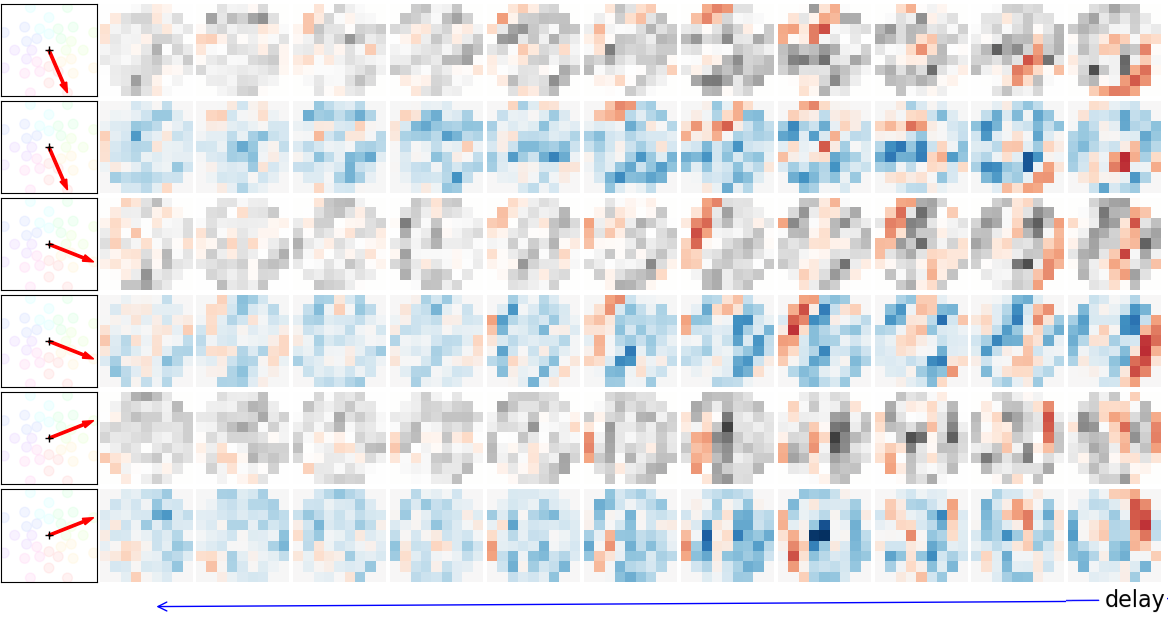
\includegraphics[width=\linewidth]{figures/motion_kernels.png}%pdf}
    }
    %\vspace{-.5cm}
    \caption{
    	Representation of the weights for $3$ of the $32$ different learned kernels of the model as learned on natural scenes. Each pair of line correspond to the OFF and ON polarities respectively, with excitatory weights in warm colors. Delays are represented in the horizontal axis from right (zero delay) to the left (delay of $11$ steps). Because of the symmetry observed between the ON and OFF event streams, we observed that kernels are very similar for the ON polarities. These weights are associated to a specific delay on the \textit{delays} axis and to a presynaptic address defined on the two other axes. %	For the sake of clarity, the values in range $[-0.05, 0.05]$ are not shown. 
	Different kernels are selective to the different motion directions and we observe some level of orientation selectivity, where ON and OFF subfields organized in a push-pull organization. 
%        One sees positive (excitatory) coefficients for the specific direction of motion but also negative (inhibitory) coefficients for other directions.
	}
    \label{fig:kernels}
\end{figure*} 
%
%
After training our model, we first analyze the weights learned for the different neurons (\seeFig{kernels}). 
We first observed a high dependence between the weights reaching the ON polarities and that reaching the OFF polarities. In particular, whenever a weight for a given position and delay is positive for one polarity, it will be negative in the other. This property comes from the way the events are generated and that the luminance can not at the same time increase and decrease. %ith the negative weights, one can observe an anti-selectivity for directions that do not correspond to the motion to which the kernel is selective to. 
We also observe that these cells show an orientation selectivity, similar to that observed in MT neurons~\citep{deangelis_functional_1999}. Interestingly, the relative organization of the receptive fields in quadrature of phase follows a push-pull organization predicted by~\citet{kremkow_push-pull_2016} to explain neurophysiological results~\citep{baudot_animation_2013}.  
Focusing on the positive weights, a strong selectivity is observed along specific axes of motion for each of the different kernels. These directions can be easily associated to the direction of motion controlled in the natural images. For instance, the first kernel shows a strong selectivity to horizontal motion directions.
%
%This qualitative look at the 3D kernels allows the reader to infer for the $8$ different motion directions used to generate our synthetic event streams.

If one focuses on the interpretation of these kernels in terms of spatio-temporal motifs embedded in the event stream, it can lead to interesting outcomes. In~\citep{grimaldi_robust_2022}, a link between event-based MLR training and Hebbian learning is drawn, allowing to say that the present model will learn its weights according to a presynaptic activity associated to the different motion directions. Each neuron becomes selective to a specific motion direction through the learning of an associated prototypical spatio-temporal spike motif. Each voxel in the 3D kernels defines a specific timestamp and a specific address. Consequently, our model is able to detect precise spatio-temporal motifs embedded in the spike train and associated to the different motion directions. The cone shape for the positive weights distribution highlights a loss of precision for longer delays, i.e. events away in the past. For the directions not coherent to the class of a training sample, an anti-Hebbian learning is also observed through the negative weights in the kernels of Figure~\ref{fig:kernels}. 

%
% \note{kernel size has to be adapted to the characteristics of motion see Samonds %~\citep{samonds}
% say that we have tested }
% \note{tester la meme expe faite par baudot et modelisée par kremkow en montrant des raster plots du modele avec NI versus Gratings }

%%%-----------------------------------------------------------------
%
\subsection{Testing with natural-like textures}
%%%-----------------------------------------------------------------
To test our model, we will quantify its ability to categorize different motions. Before applying the model on natural images, we will first test the model on simpler, parameterized stimuli. In that order, we use a set of synthetic visual stimuli, \textit{Motion Clouds}~\citep{leon_motion_2012} which are natural-like random textures for which we can control for velocity, among other parameters (\seeFig{motion_clouds})~\citep{vacher_bayesian_2018}. In particular, we will set the spatial size and duration similarly to the motion task defined above.
This procedure defines a set of textures with different spatial properties and different motions $\va{v}_k$ with  $1 \le k \le \Nclass$ and $\Nclass=8$ defined by a constant speed and linearly spaced directions $
\speed_\kernelind = 
  ( 
    \speed \cdot \cos(2\pi\cdot \frac{\kernelind}{\Nspeed}),
    \speed \cdot \sin(2\pi\cdot \frac{\kernelind}{\Nspeed})
  )
$.
For any given velocity, we also varied the parameters of the textures, such as the mean and variance of the orientation or spatial frequency content to provide with some naturalistic variability. This method provides a rich dataset of textured movies for which we know the ground truth for motion.
%%%-----------------------------------------------------------------
%: fig:motion_clouds
%%%-----------------------------------------------------------------
\begin{figure}%[h!]
    \centering
    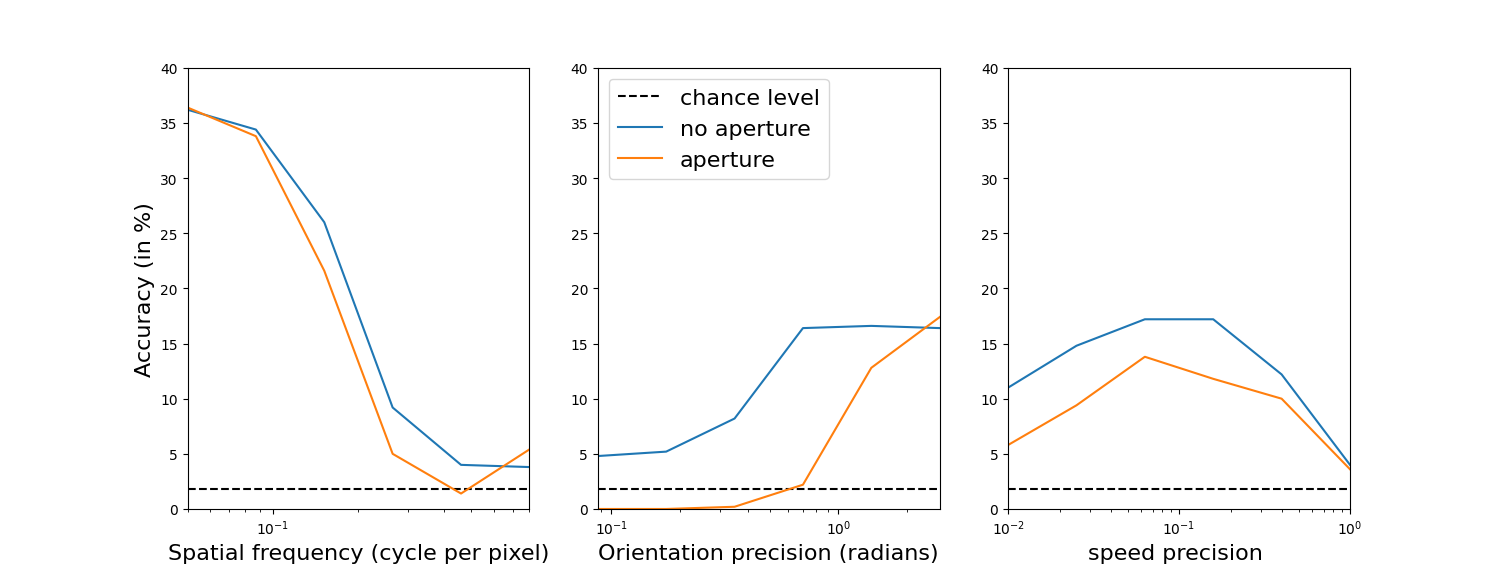
\includegraphics[width=0.99\linewidth]{figures/2022-09-27_MotionDetection_motion_clouds.png}%motion_clouds.pdf} % 2022-09-27_MotionDetection_motion_clouds.png}%
    \caption{{\bf Role of stimulus parameters in the motion detection accuracy.} Accuracy as a function of {\bf (a)} the mean spatial frequency, {\bf (b)} the bandwidth in orientation: from a grating-like (left) to isotropic textures (right)), {\bf (c)} the bandwidth in speed, from a rigid motion (left) to independent frames (right). Note that these accuracy is computed both in the case where orientation of the synthetic texture is necessarily perpendicular to the motion (no aperture) or arbitrary (aperture), showing that accuracy decreases in the latter case.}
    \label{fig:motion_clouds}
\end{figure}
%%%-----------------------------------------------------------------

We plot here main axis of interests. First, as we change the mean spatial frequency of the texture, we observe a monotonous decrease in accuracy. This comes as a similar trend as that observed in the primary visual areas~\citep{priebe_tuning_2006}. %\note{we should really do something more serious here...} 
Notably, the accuracy is better for a large spatial frequency bandwidth (which qualitatively resemble a more textured stimulus) than for a grating-like stimulation, reminiscent to the behavioral response of humans' eye movements to such stimuli~\citep{simoncini_more_2012}. Interestingly, we also see a modulation of accuracy as a function of orientation bandwidth. When the stimulus is grating-like and that the orientation is arbitrary with respect to the direction of motion, the system is faced with the aperture problem and see a decrease of accuracy. This is not the case for isotropic stimuli or when the orientation is perpendicular to the direction of motion. Finally, we manipulated the amount of change between two successive frames, similar to a temperature parameter. This shows a progressive decrease in accuracy, similar to that observed in the amplitude of humans' eye movements~\citep{mansour_pour_speed_2018} but also that accuracy is low for a rigid motion which lacks variability.
%
\subsection{Accuracy efficiency trade-off}% for the motion detection task}
%%%-----------------------------------------------------------------

Once our MLR is trained, we obtain spatio-temporal kernels corresponding to the weights associated to the heterogeneous delays of our layer of spiking neurons and which may be used for detection. We observed that the distribution of the kernels' weights is sparse, with most values near zero. As shown in the formalization of our event-based model, the computational cost of our model if implemented on a neuromorphic chip would be dominated by the number of spikes times the number of synapses. Indeed, the computations are dominated by the convolution operation. In a dense setting, this corresponds for all voxels in the output to a sum over all voxels in the inputs for all weights in the kernel. If the support of information is sparse, then computations can be performed only on those events. Also, if we set some weights of the kernels to zero, then the sum can be skipped for those addresses. Knowing the sparseness of the input, the total number of computations thus scales with the number of nonzero synaptic weights. 

To assess the robustness of the classification as a function of the computational load, we will prune the weights in $\{\synapse_\ranksyn\}_{\ranksyn \in [0,\Nsyn)}$ that are below a defined threshold. In Figure~\ref{fig:accuracy}, we plot the classification accuracy as a function of the relative number of computations, or active weights, per decision for each neuron of the layer. As a comparison and to account for the gain in performance by using heterogeneous delays, we provide the accuracy obtained with a MLR model using 2D time surface (in red) as in~\citep{grimaldi_robust_2022}. This latter method is based on delays from the last recorded events and uses fewer computations (in our case $15\times15$) than the dense 3D kernels without any pruning ($15\times15\times8$). While less computations are needed, the classification performance obtained for the model using time surfaces is similar to our method using all the weights of the kernels.

By pruning weights, we observe that the evolution of accuracy as a function of the log percentage of active weights fits well a sigmoid curve. Half-saturation level is reached at about $3.5\times 10^{-3}\%$ of active weights, corresponding in our setting to a total amount of $6$ computations per decision. Compared to the full kernels, the accuracy of our method is maintained to its top performances when dividing the number of computations by a factor up to about $200$. In this case, the number of computations is greatly reduced compared to~\citep{grimaldi_robust_2022}, thus demonstrating the efficiency of the presented method. 

%
%%%-----------------------------------------------------------------
%: fig:accuracy
%%%-----------------------------------------------------------------
\begin{figure}%[h!]
    \centering
    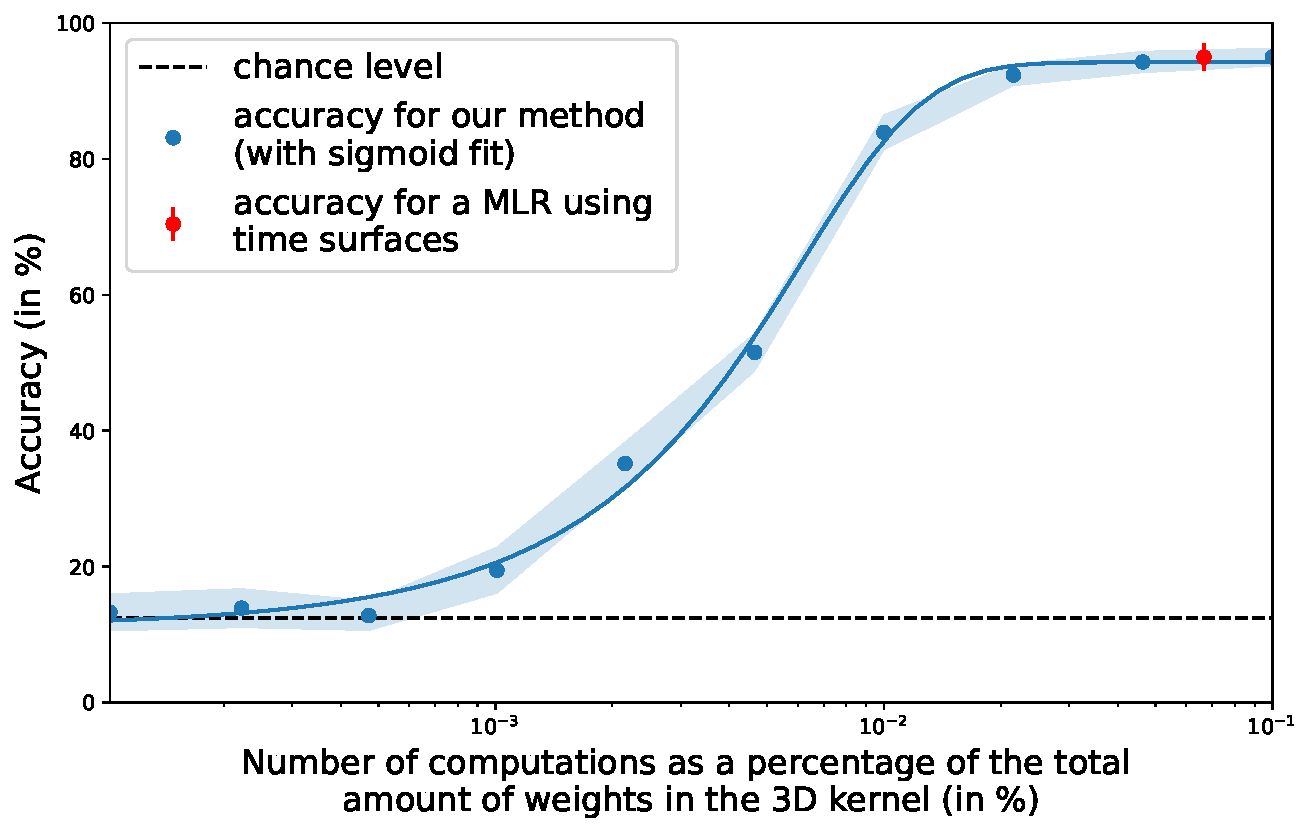
\includegraphics[width=0.95\linewidth]{figures/accuracy.pdf}
    \caption{Accuracy as a function of the number of computation load for the model with heterogeneous delays (blue line) and for a method using 2D time surfaces (red dot)~\citep{grimaldi_robust_2022}. The relative computational load (on a log axis) is controlled by changing the percentage of active weights relative to the dense convolution kernel. We observe a similar accuracy than HOTS, yet that our model could achieve a similar accuracy with significantly fewer coefficients.}
    \label{fig:accuracy}
\end{figure}

% \note{try also a quantization of the weights (binary?)}
%
\section{Discussion}
%%%-----------------------------------------------------------------
%%%-----------------------------------------------------------------
In this paper, we have introduced a generic SNN with heterogeneous delays and shown how it compares favorably to a state-of-the-art event-based classification algorithm for a visual motion detection task. The learned model shares a number of similarities with neurobiological anatomical observations, as well as with behavioral results. The event-based computations of our method can be drastically reduced by pruning synapses, while maintaining top classification performance. This shows that we can take advantage of the precise timing of spikes to improve the performance of neural computations.
%
\subsection{Synthesis and main contributions}
%%%-----------------------------------------------------------------
In summary, in this paper we have presented a HD-SNN model that has been trained and evaluated on a complex motion detection task. The model has been defined to provide optimal detection of event-driven spatio-temporal motifs. We have shown that the model, when trained on a dataset of natural images with realistic eye movements, learns kernels similar to those found in the early visual cortex. We then demonstrated that the model shows similarities to biological responses. We have evaluated the computational cost of this model when implemented in a setting similar to event-based hardware. We show that the use of heterogeneous delays may be an efficient computational solution for future neuromorphic hardware, but also a key to understanding why spikes are a universal component of neural information processing.

We would like to highlight a few innovations in the contributions that are presented in this paper. First, whereas~\citep{ghosh_spatiotemporal_2019,yu_stsc-snn_2022} use a correlation-based heuristic, which we observed to be less efficient, the generic heterogeneous model is formalized from first principles for optimal detection of the event-based spatio-temporal motifs. Moreover, in comparison to HOTS~\citep{lagorce_hots_2017}, the weights are explicable as they directly inform on the logit (inverse sigmoid of the probability) of detection of each spatio-temporal spike motif. Another novelty is that the model learns the weights and the delays simultaneously. For example, the polychronization model~\citep{izhikevich_polychronization_2006} learns only the weights using STDP, while the delays are randomly drawn and their values are frozen during learning. In addition, the model is evaluated on a realistic task, while models such as the tempotron are tested on simplified toy problems~\citep{gutig_tempotron_2006}. Another major contribution is to provide a model that is suitable for learning any kind of spatio-temporal spiking motifs and that can be trained in a supervised manner by providing a dataset of supervision pairs. Instead of relying on a careful description of the physical rules governing a task, e.g. the luminance conservation principle for motion detection~\citep{benosman_asynchronous_2012, dardelet_event-by-event_2021}, this allows a more flexible definition of the model using this properly labeled dataset.
%
\subsection{Main limits}
%%%-----------------------------------------------------------------
We have identified a number of limitations of our model, which we will now discuss in detail. First, the entire framework is based on a discrete binning of time, which is not compatible with the continuous nature of biological time. We used this binning to efficiently implement the framework on conventional hardware, especially GPUs, to be able to use fast three-dimensional convolutions. We have tested the effect of the width of the time bin and shown that it has essentially no effect on the results presented in this paper. This is consistent with the relative robustness of other event-based frameworks such as HOTS~\citep{lagorce_hots_2017}, where accuracy was unaffected when the input spikes were subjected to noisy perturbations up to $1~\ms$~\citep{grimaldi_robust_2022}. This suggests the possibility of analytically including a precision term in the temporal value of the input spikes. This mechanism may be implemented by the filtering implemented by the synaptic time constant of about $5~\ms$. Furthermore, it is possible to circumvent the need for time discretization by the use of a purely event-based scheme. In fact, it is not necessary to compute the voltage traces between two spikes~\citep{hanuschkin_general_2010}. Thus, it is possible to define a purely event-based framework. Such an architecture could provide promising computational speedups. % \note{pourrait parler du poster bernstein? de nadafian?}

A further limitation is that the model is purely feed-forward. Thus, the spikes generated by the postsynaptic neurons are based solely on information contained in the classical receptive field. However, it is well known that neurons in the same layer can interact with each other using lateral interactions, for example in V1, and that this can be the basis for computational principles~\citep{chavane_revisiting_2022}. For example, the combination of neighboring orientations may contribute to image categorization~\citep{perrinet_edge_2015}. Furthermore, neural information is modulated by feedback information, e.g. to distinguish a figure from its background~\citep{roelfsema_early_2016}. Feedback has been shown to be essential for building realistic models of primary visual areas~\citep{boutin_sparse_2020, boutin_effect_2020}, especially to explain non-linear mechanisms~\citep{boutin_pooling_2022}. Currently, mainly due to our use of convolutions, it is not possible to implement these recurrent connections in our implementation (lateral or feedback). However, by inserting new spikes into the list of spikes reaching presynaptic addresses, the generic model is able to incorporate them. While theoretically possible, this needs to be properly adjusted in practice so that these recurrent connections do not amplify neuronal activity outside a homeostatic state (by extinction or explosion).
% \note{ dire que la prédiction permet de faire de la prediction et que ça explique les résultats de leBec}%~\citep{perrinet_motion-based_2012}

Such recurrent activity would be essential for the implementation of predictive or anticipatory processes. This is essential in a neural system because it contains several different delays that require temporal alignment~\citep{hogendoorn_predictive_2019}. This has been modeled before to explain, for example, the flash-lag illusion~\citep{khoei_flash-lag_2017}. %\note{Say that this could be implemented by properly setting the timing of the label} 
As mentioned previously, this could be implemented using generalized coordinates (i.e., variables such as position complemented by velocity, acceleration, jerk,~\ldots), and ``neurobiologically, using delay operators just means changing synaptic connection strengths to take different mixtures of generalized sensations and their prediction errors''~\citep{perrinet_active_2014}. Our proposed model using heterogeneous delays provides an alternative and elegant implementation solution to this problem.
%
\subsection{Perspectives}
%%%-----------------------------------------------------------------
% \note{la tache ne met pas en avant les capacites des motifs hetero synaptiques =trop simple et peut se faire en HOTS}
In defining our task, we emphasized that the generation of events depends on the spatial gradient in each image. This gradient has both horizontal and vertical dimensions, and its maxima are generally orientation dependent. Taken together, these oriented edges form the contours of visual objects in the scene~\citep{koenderink_representation_1987}. Thus, there is an interdependence between the information about motion and the information about orientation within the event stream. It would be crucial to investigate this dependency further. This could be initiated by training the model on a dataset with labels that provide local orientation. %\note{we can say that we tried it and that it works well}. 
Exploring this dependence will allow us to dissociate these two forms of visual information and enable us to integrate them. In particular, it will allow us to consider that the definition of motion is more accurate perpendicular to an oriented contour (aka the aperture problem). Thus, it will allow us to implement recurrent prediction rules, such as those identified to dissociate this problem~\citep{perrinet_motion-based_2012}.

The model is trained on a low-level local motion detection task, and one might wonder if it could be trained on higher-level tasks. An example of such a task would be the estimation of depth in the visual scene. There are several sources of information for depth estimation, such as binocular disparity or changes in texture or shading, but in our case motion parallax would be the most important cue~\citep{rogers_motion_1979}. This is because objects that are close to an observer will move relatively faster on the retina than an object that is far away, and also because visual occlusions are dependent on the depth order. Using this information, it is possible to segment objects and estimate their depth~\citep{yoonessi_contribution_2011}. However, this would require the computation of the optical flow first, i.e., the extension of the framework described here for a rigid full-field motion to a more general one where the motion may vary in the visual field. A possible implementation is therefore to add a new layer to our model, analogous to the hierarchical organization highlighted in the visual cortex. This is theoretically possible by using the output of our model (which estimates velocity in retinotopic space) as input to a new layer of neurons that would estimate velocity in the visual field, including the depth dimension in the output supervision labels. This could have direct and important applications, e.g. in autonomous driving to detect obstacles in a fast and robust way. Another extension would be to actively generate sensor motion (physical or virtual) to obtain better depth estimates, especially to disambiguate uncertain estimates~\citep{nawrot_eye_2003}.

In conclusion, the model that we have presented provides a way to process event-based signals in an efficient manner. We have shown that we can train the model semi-supervised, knowing \emph{what} output label, but not \emph{when} it occurs. Another perspective would be to extend the model to a fully self-supervised learning paradigm, i.e., without any labeled data~\citep{barlow_unsupervised_1989}. This type of learning is thought to be prevalent in the central nervous system and, assuming the signal is sparse~\citep{olshausen_emergence_1996}, one could extend these Hebbian sparse learning schemes to spikes~\citep{perrinet_emergence_2004, masquelier_competitive_2009}. We expect that this would be particularly useful for exploring neurobiological data. Indeed, there is a large literature showing that brain dynamics often organize into stereotyped sequences, such as synfire chains~\citep{ikegaya_synfire_2004}, packets~\citep{luczak_sequential_2007}, or hippocampal sequences~\citep{pastalkova_internally_2008, villette_internally_2015}. These patterns are stereotyped and robust, as they can be activated in the same pattern from day to day~\citep{haimerl_internal_2019}. In contrast to conventional methods of processing neurobiological data, such an event-based model would be able to answer key questions about the representation of information in neurobiological data, and it would open up possibilities in the field of computational neuroscience. Furthermore, it would open up possibilities in the field of machine learning, especially in computer vision, to address current key concerns such as robustness to attacks, scalability, interpretability, or energy consumption.
%
%%%%%%%%%%%%%%%%%%%%%%%%
\backmatter
%
\bmhead{Acknowledgments}
%
% Acknowledgement hidden for review.
\Acknowledgments
%
%%%%%%%%%%%%%%%%%%%%%%%%

\section*{Statements and Declarations}

\paragraph{Funding}

\Funding %

\paragraph{Conflict of interest}
Not applicable.
% The authors do not have any financial or non-financial interests directly or indirectly related to this work.

\paragraph{Ethics approval}
Not applicable.

\paragraph{Consent to participate}
Not applicable.

\paragraph{Consent for publication}
Not applicable.

\paragraph{Availability of data and materials}
Not applicable.

\paragraph{Code availability}
%
The code is publicly available online at: \url{https://github.com/SpikeAI/pyTERtorch}.
%   
\paragraph{Authors' contributions}
%
Both authors contributed to the conceptualization and methodology design of the study, to the project's coordination and administration. Laurent Perrinet carried out the funding acquisition and supervision. Formal analysis and investigation were performed by both authors. Results visualization and presentation were realized by both authors. The manuscript was written by both authors. Both authors have read and approved the final manuscript.
%%%%%%%%%%%%%%%%%%%%%%%%
\bibliographystyle{apalike}
\bibliography{FastMotionDetection}
\end{document}
%%%%%%%%%%%%%%%%%%%%%%%%